\documentclass{article}
\usepackage{tikz,tcolorbox}
\usepackage{array} % For customizing tables
\usepackage{booktabs} % For better horizontal lines
\usepackage[a4paper, paperwidth=25cm, paperheight=25.5cm, left=2cm, right=2cm, top=2cm, bottom=2cm]{geometry}
\usepackage{multicol}
\usepackage{amsmath}
\usepackage{pgfplots}
\usepackage{makecell}
\usetikzlibrary{patterns}
\definecolor{greenPlot}{HTML}{14C877}
\definecolor{orangePlot}{HTML}{EA6E12}
\definecolor{purplePlot}{HTML}{4C12EA}
\definecolor{blueArea}{HTML}{10D9EE}
\definecolor{redPlot}{HTML}{ED014A}
\definecolor{box}{HTML}{27C1A0}
\definecolor{pur}{HTML}{A128E1}

\tcbuselibrary{skins, breakable, theorems}

\newtcolorbox{prettyBox}[2]{
  enhanced,
  colback=white!90!#2,   % Background color based on the second parameter (color)
  colframe=#2!60!black,  % Frame color based on the second parameter (color)
  coltitle=white,        % Title color (white)
  fonttitle=\bfseries\Large,
  title=#1,              % Title from the first parameter
  boxrule=1mm,
  arc=0.5mm,
  drop shadow=#2!35!gray, % Drop shadow color based on the second parameter (color)
}




\setlength{\parindent}{0pt}
\setcellgapes{3pt}  % Adjust padding as needed
\makegapedcells
\begin{document}
\renewcommand{\arrayrulewidth}{0.75mm} % Set line thickness
\setlength{\tabcolsep}{12pt} % Set horizontal padding
\renewcommand{\arraystretch}{1.5} % Set vertical padding (1.0 is default)
\exer{1}


\textbf{\underline{ex1.html}}
\vspace{0.1cm}

\lstinputlisting[style=htmlstyle]{Code/EX1/ex1.html}

\vspace{1.5cm}

\textbf{\underline{Output}}

\vspace{0.1cm}
\begin{center}
\setlength{\fboxrule}{2pt} % Set border thickness
\fbox{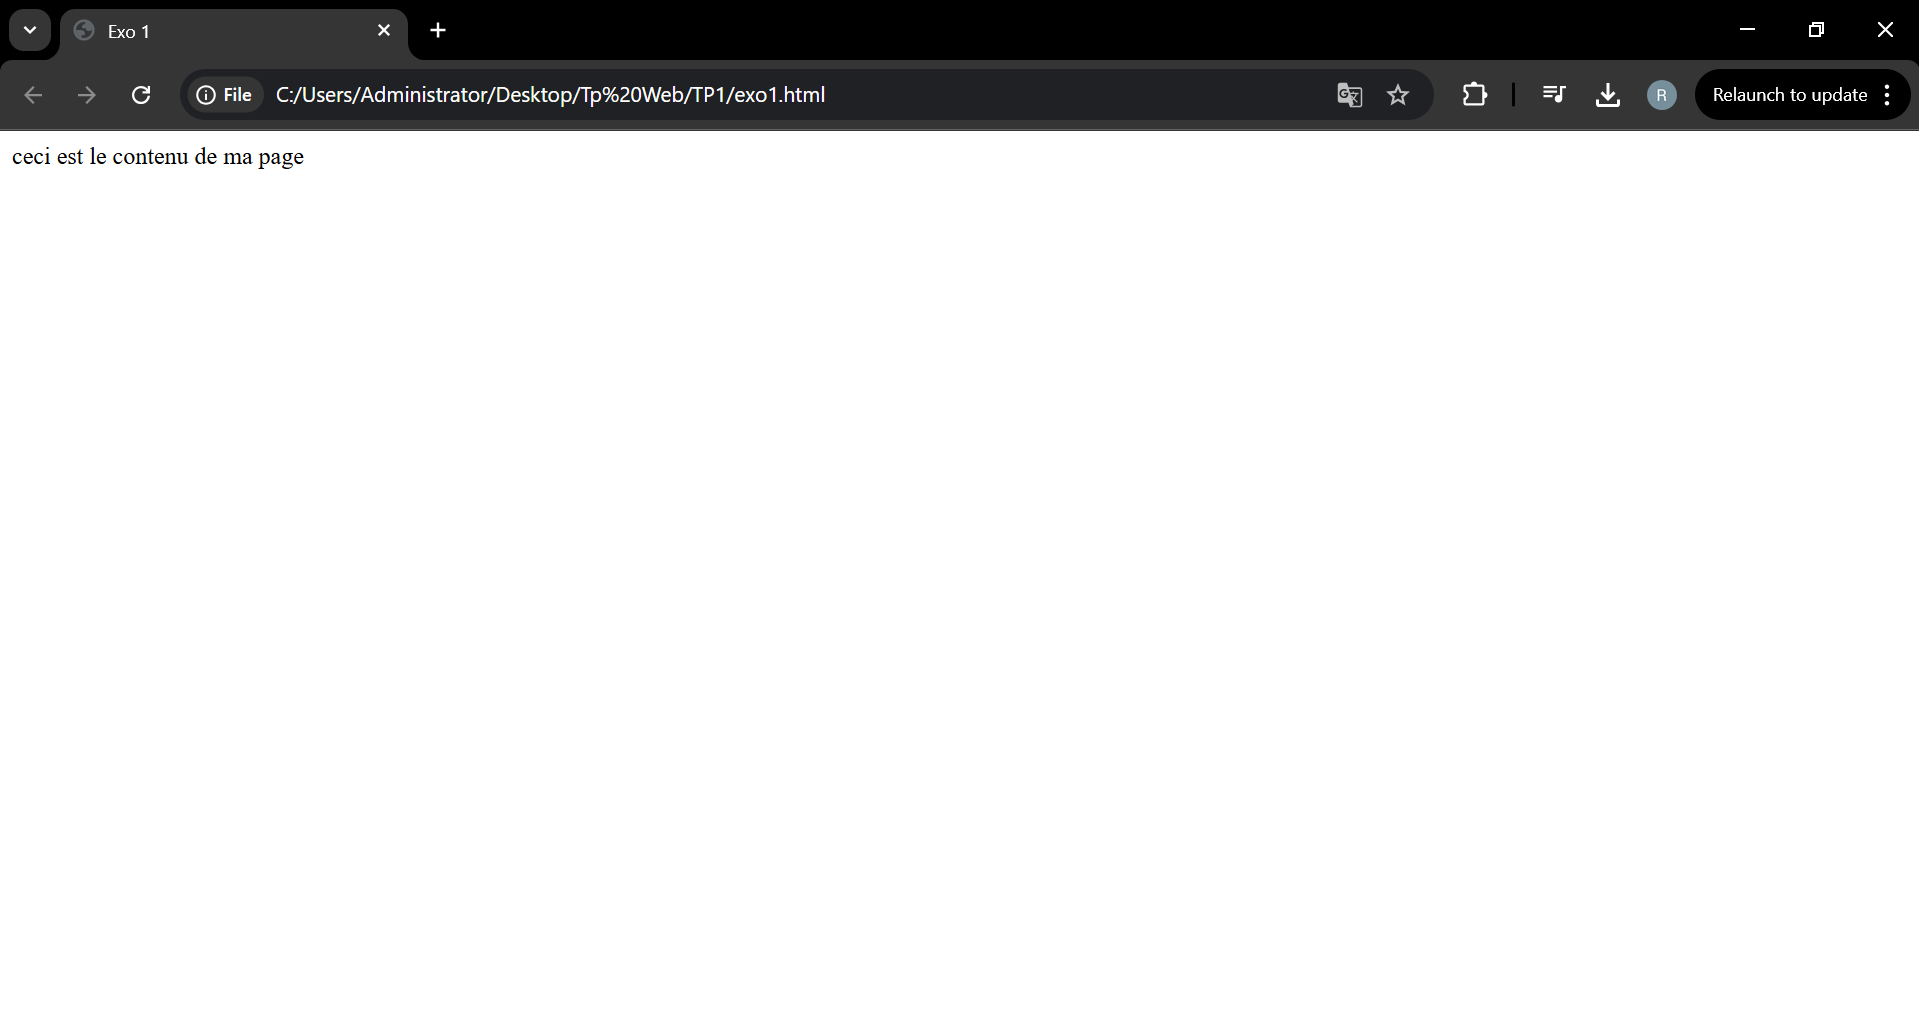
\includegraphics[height=0.4\textheight]{Code/EX1/ex1.PNG}}
\end{center}

\vspace{1cm}
\subsection*{\underline{Solution}}
\[ \text{max } Z = 6x_1 + 8x_2\]  

\[    
\left\{
    \begin{array}{l}
        6x_{1} + 3x_{2} \leq 18 \\[2pt]
        2x_{1} + 3x_{2} \leq 9 \\[2pt]
        x_{1}, x_{2} \text{ are integers}
    \end{array}
    \right.
\]

\begin{center}
    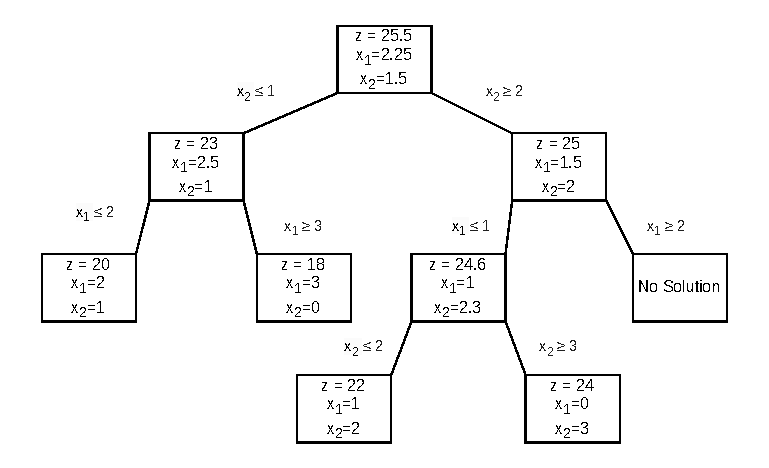
\includegraphics{Exercice/PY/EX1/b1.drawio.pdf}
\end{center}

\vspace{0.5cm}

\[\text{Optimal Solution is }\hspace{0.1cm} \boxed{(x_1,x_2) = (0,2)}\]

\begin{center}
    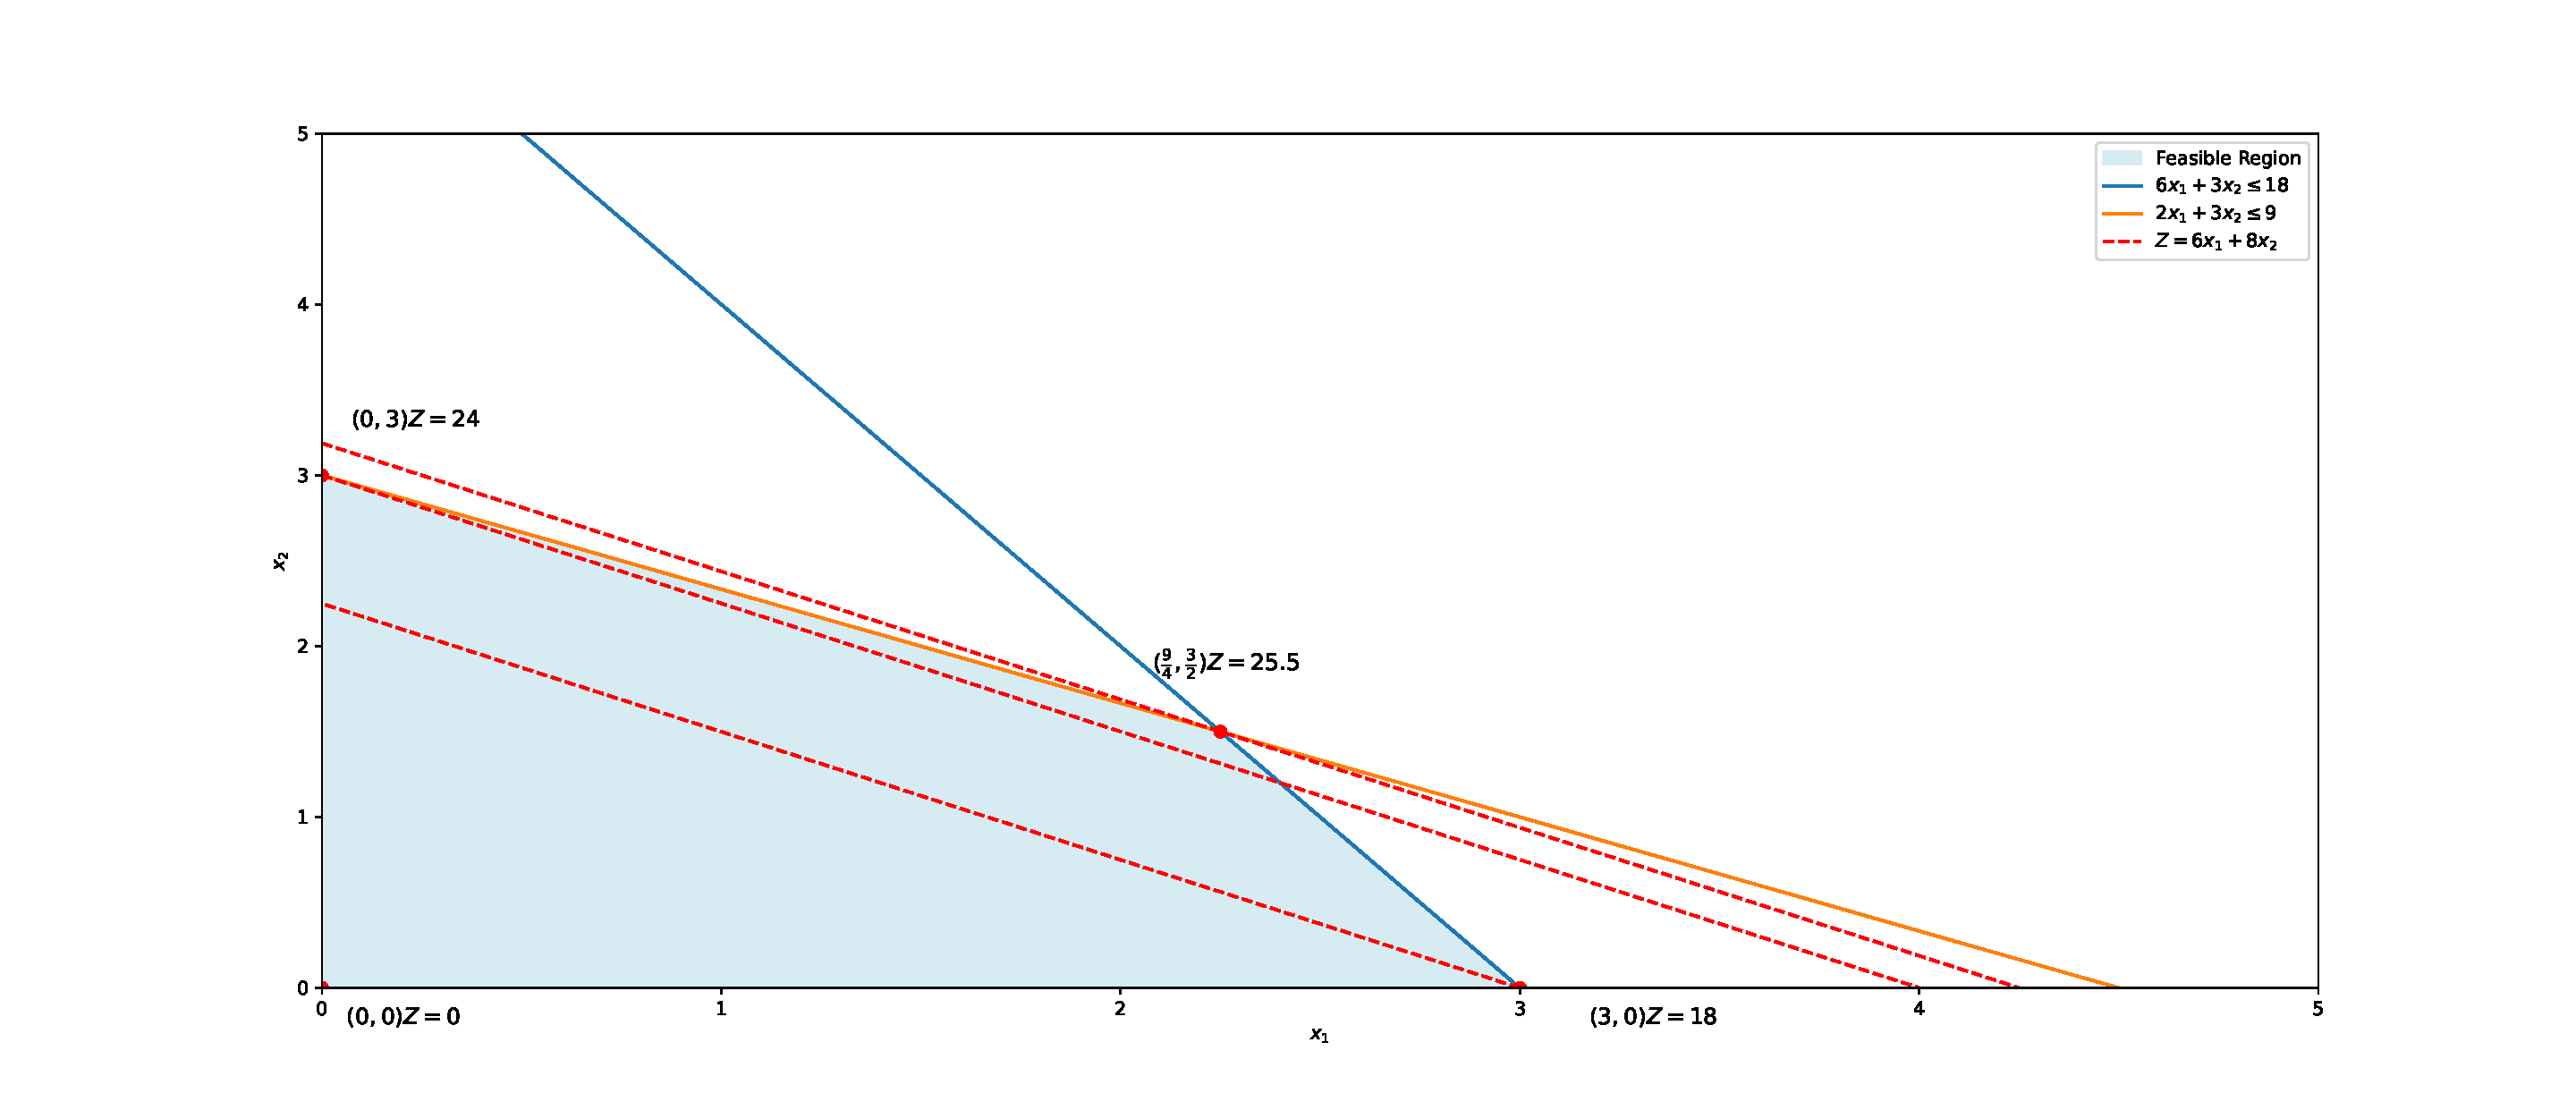
\includegraphics[width = \textwidth]{Exercice/PY/EX1/ex1.1.pdf}
\end{center}


\begin{center}
    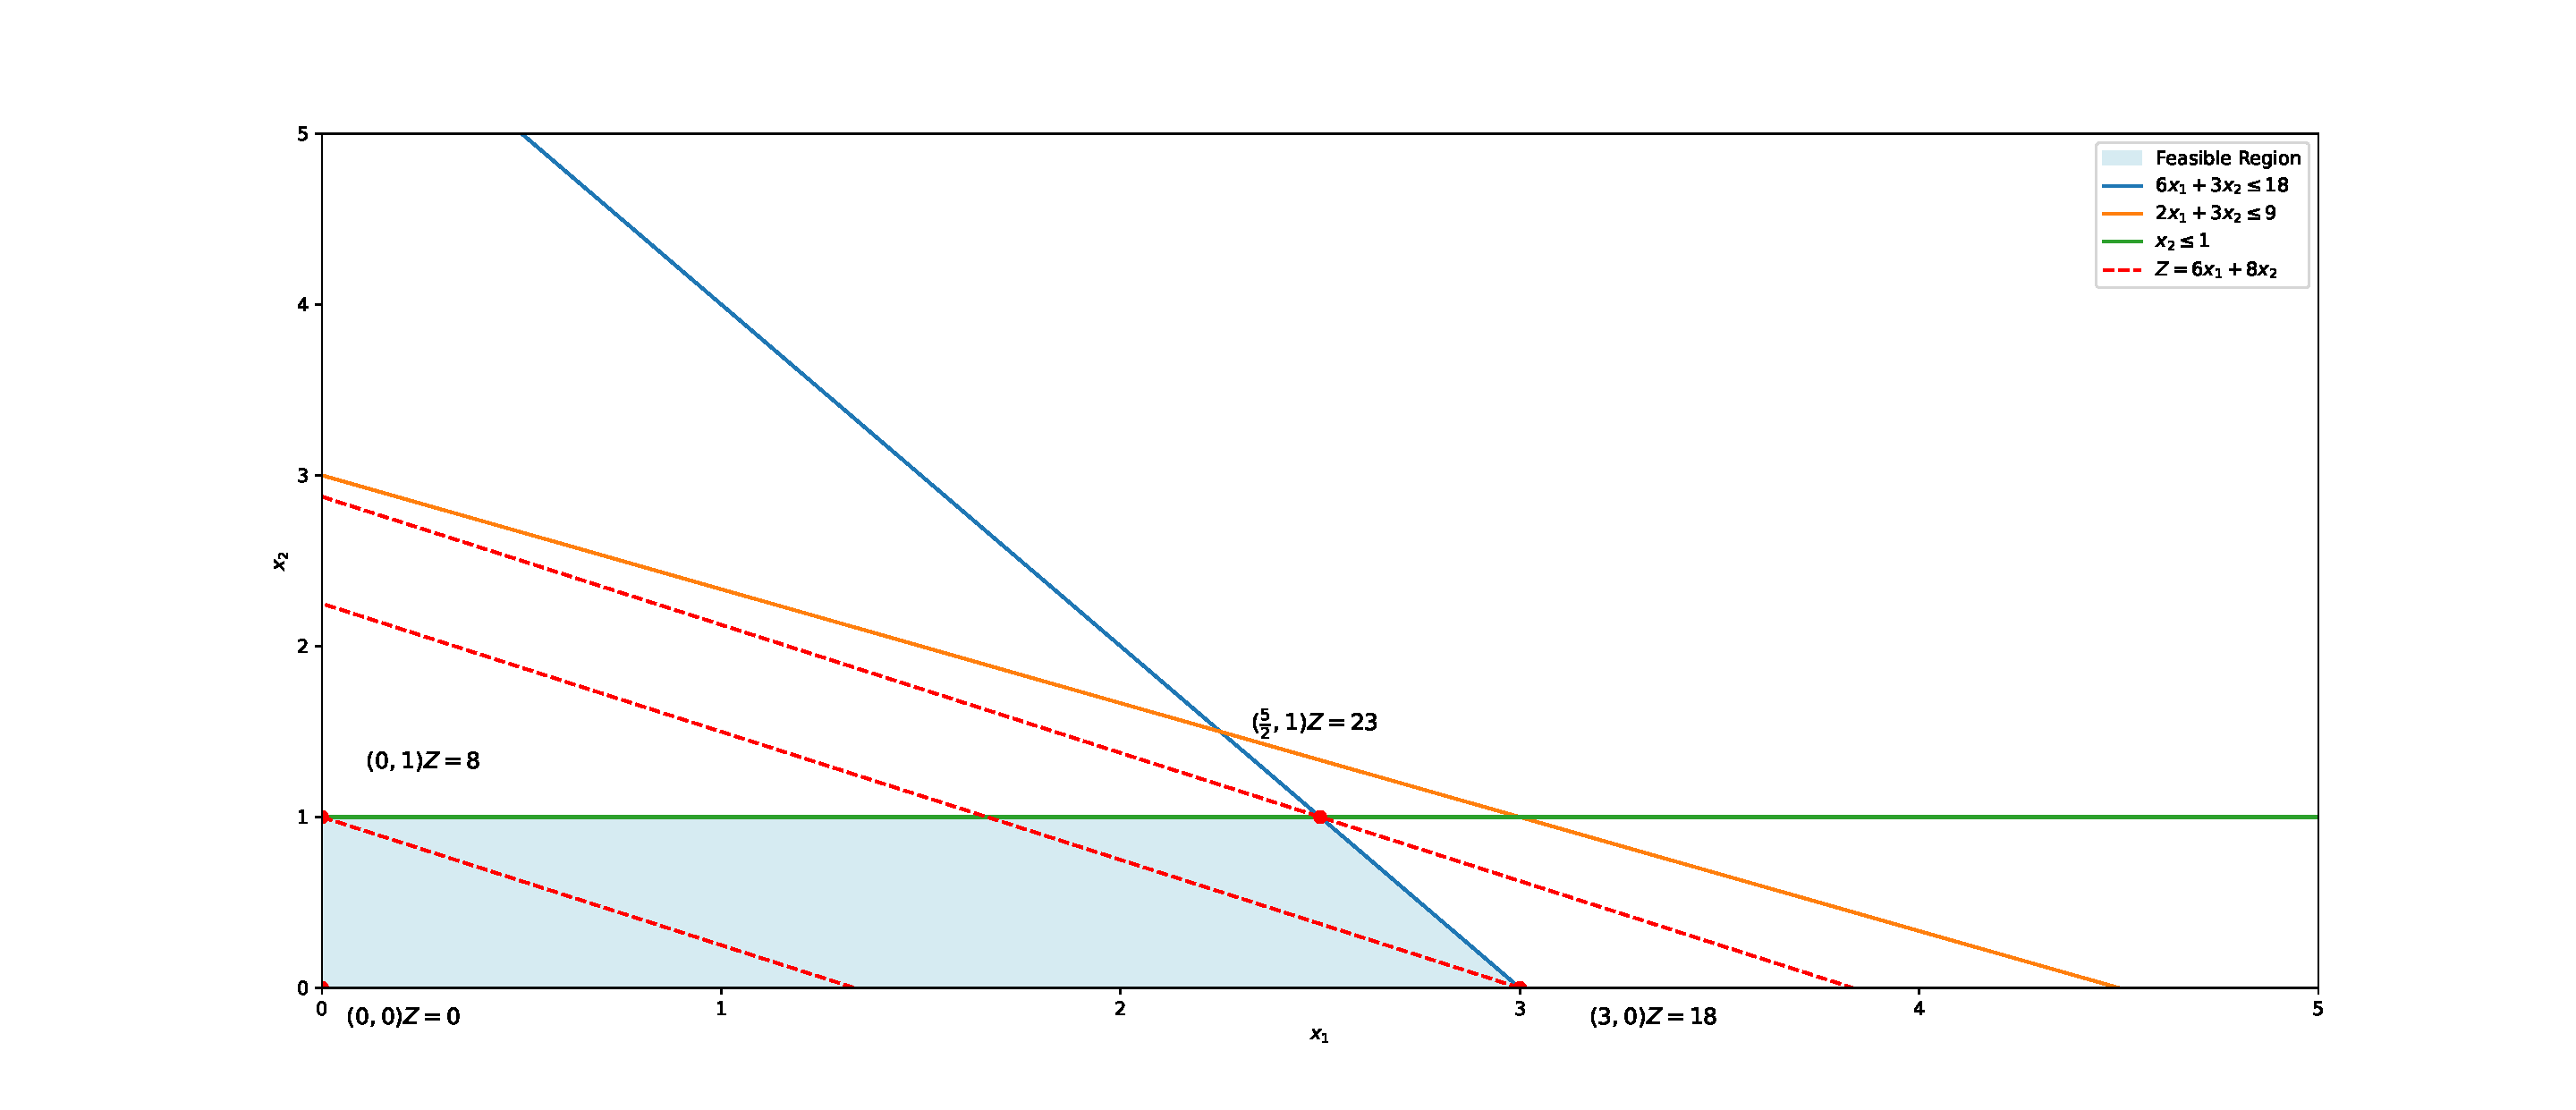
\includegraphics[width = \textwidth]{Exercice/PY/EX1/ex1.2.pdf}
\end{center}


\begin{center}
    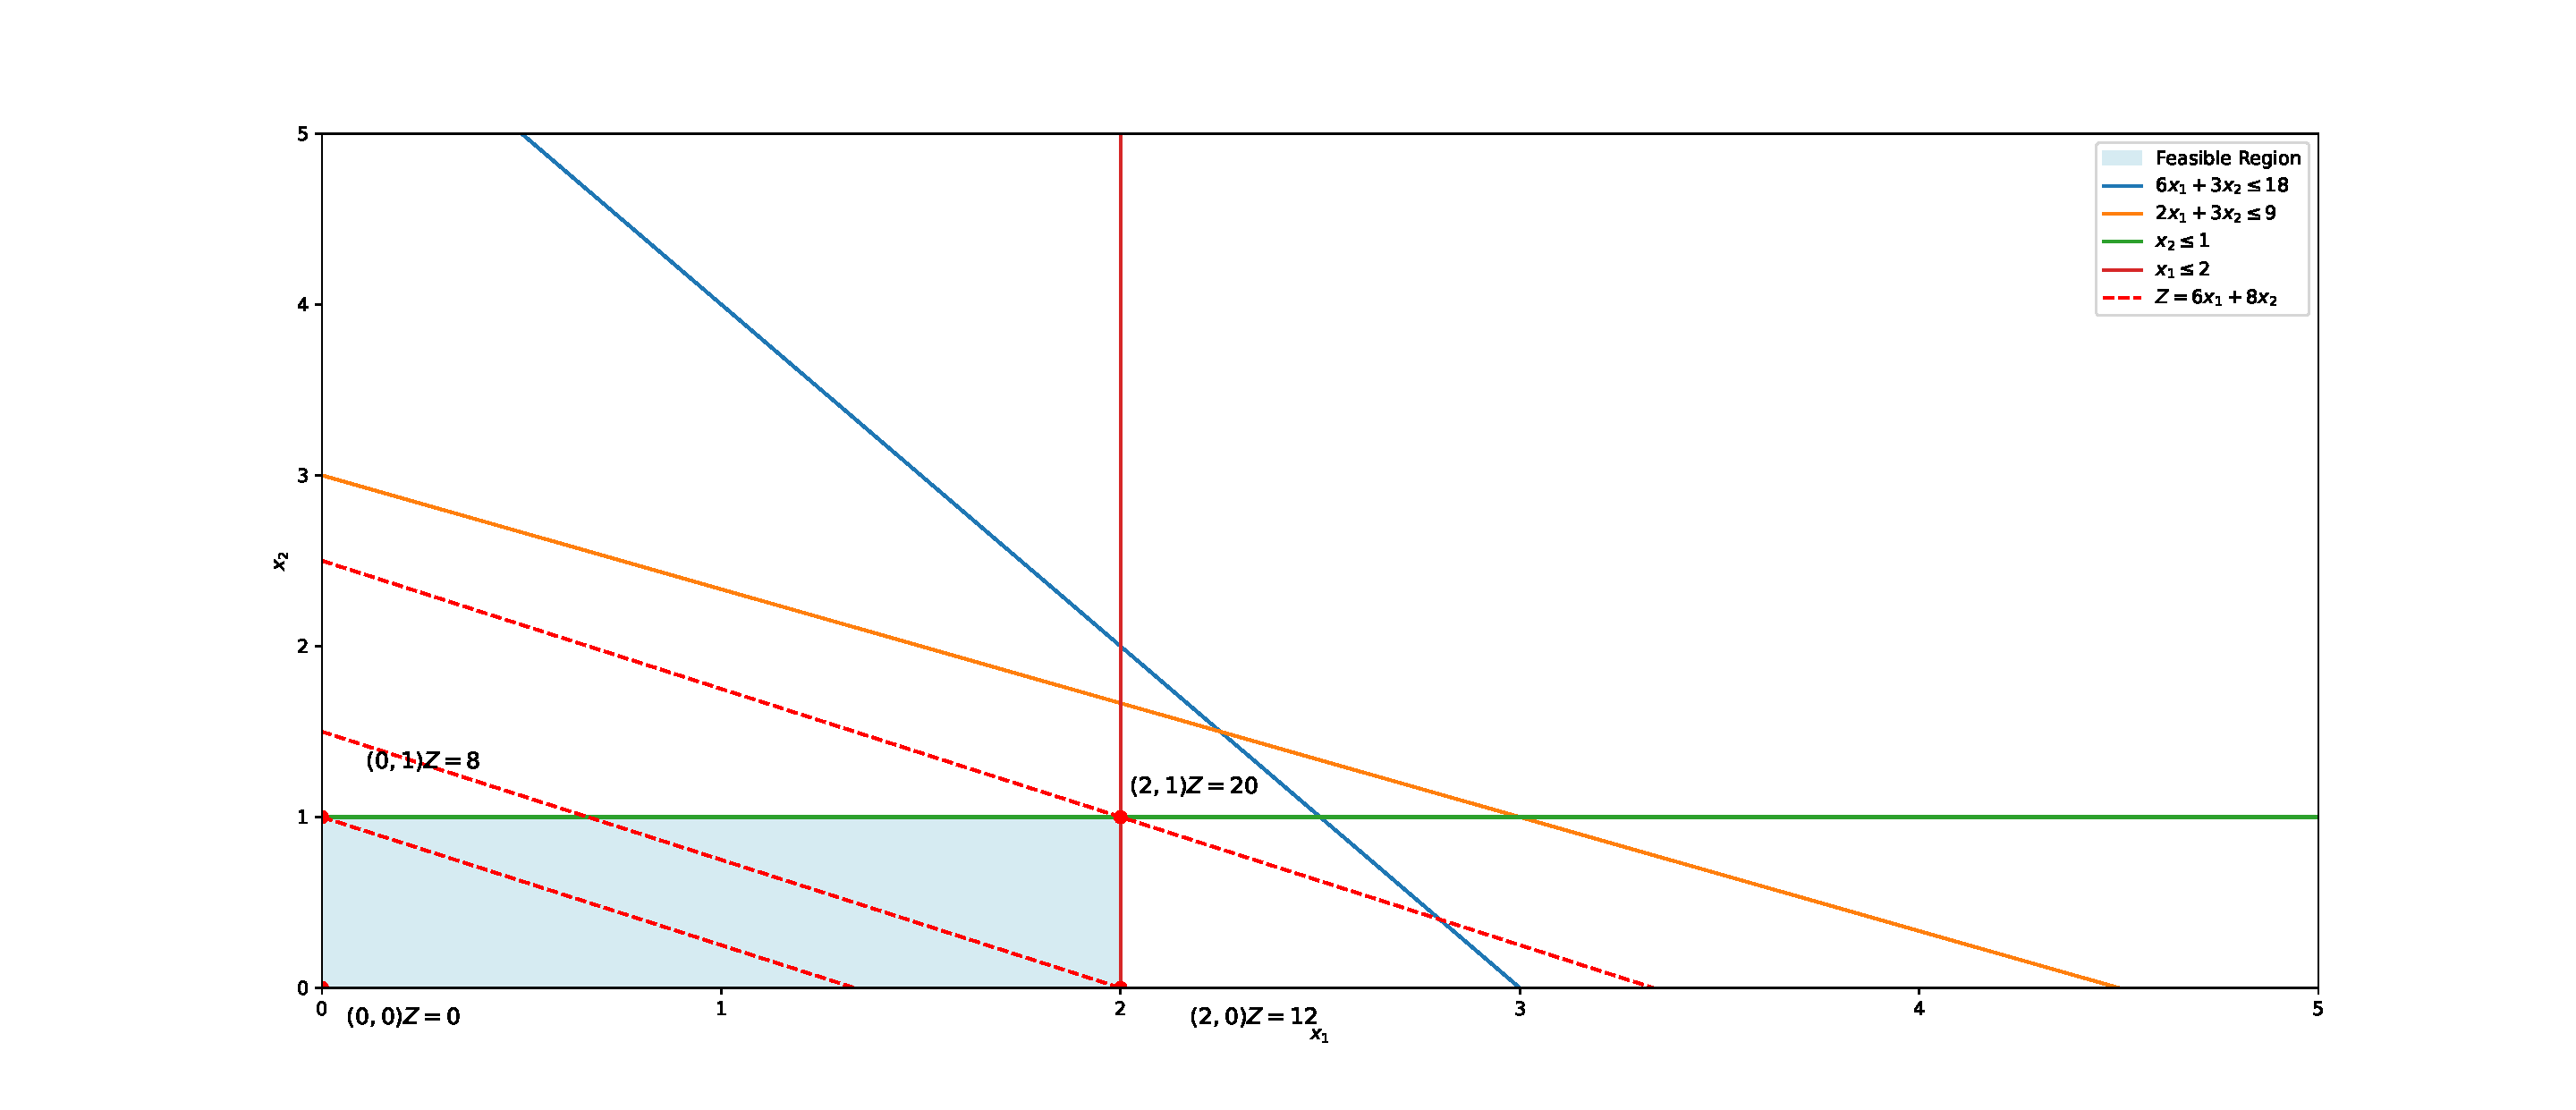
\includegraphics[width = \textwidth]{Exercice/PY/EX1/ex1.3.pdf}
\end{center}

\begin{center}
    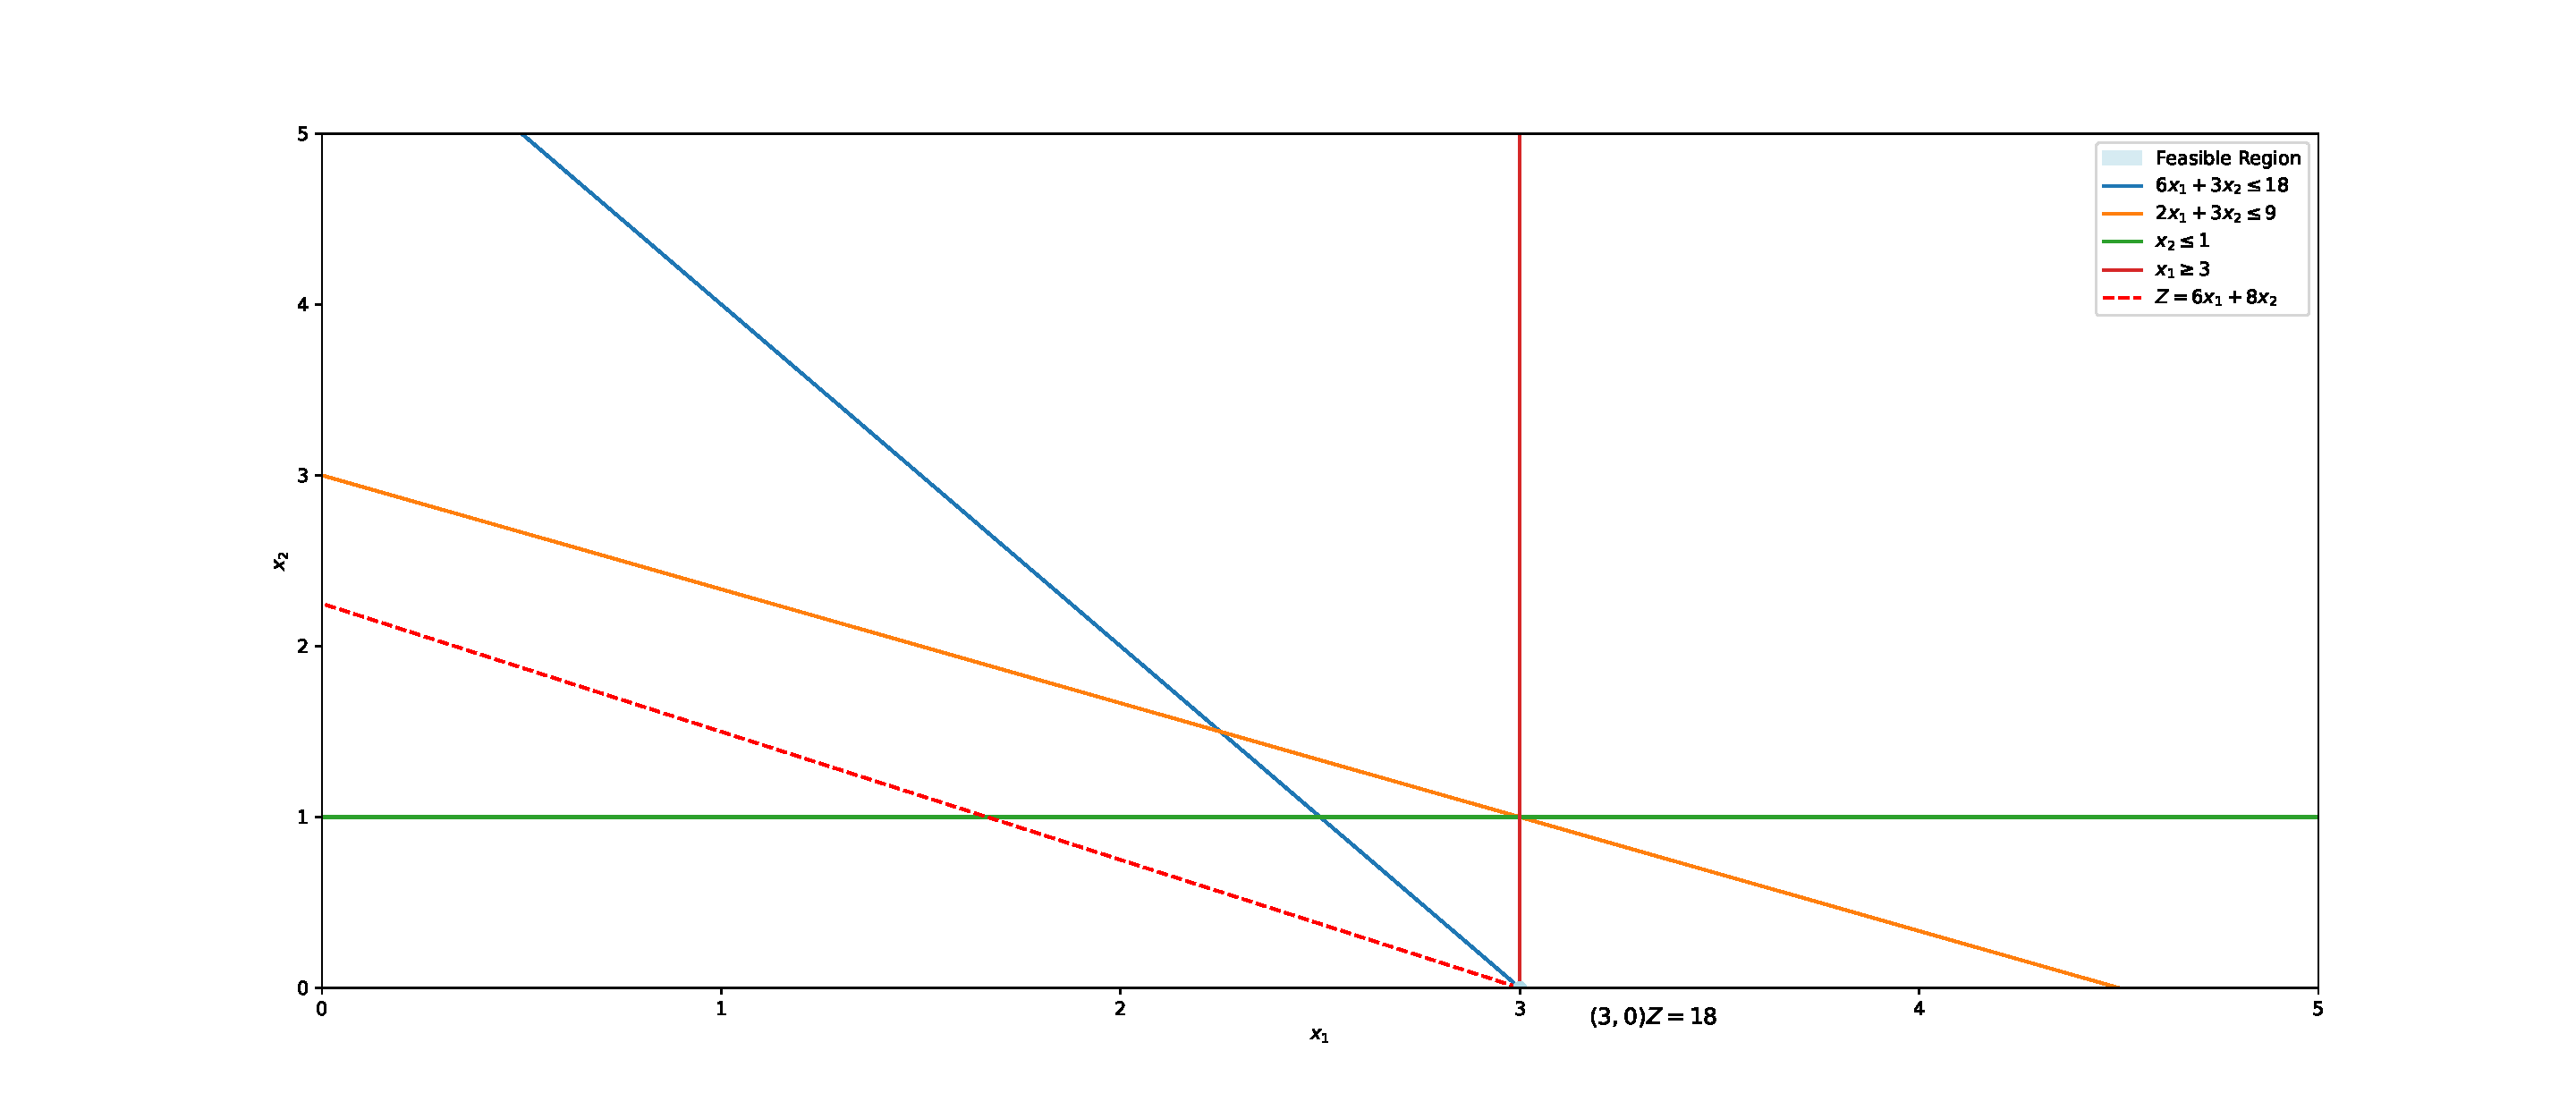
\includegraphics[width = \textwidth]{Exercice/PY/EX1/ex1.4.pdf}
\end{center}
\begin{center}
    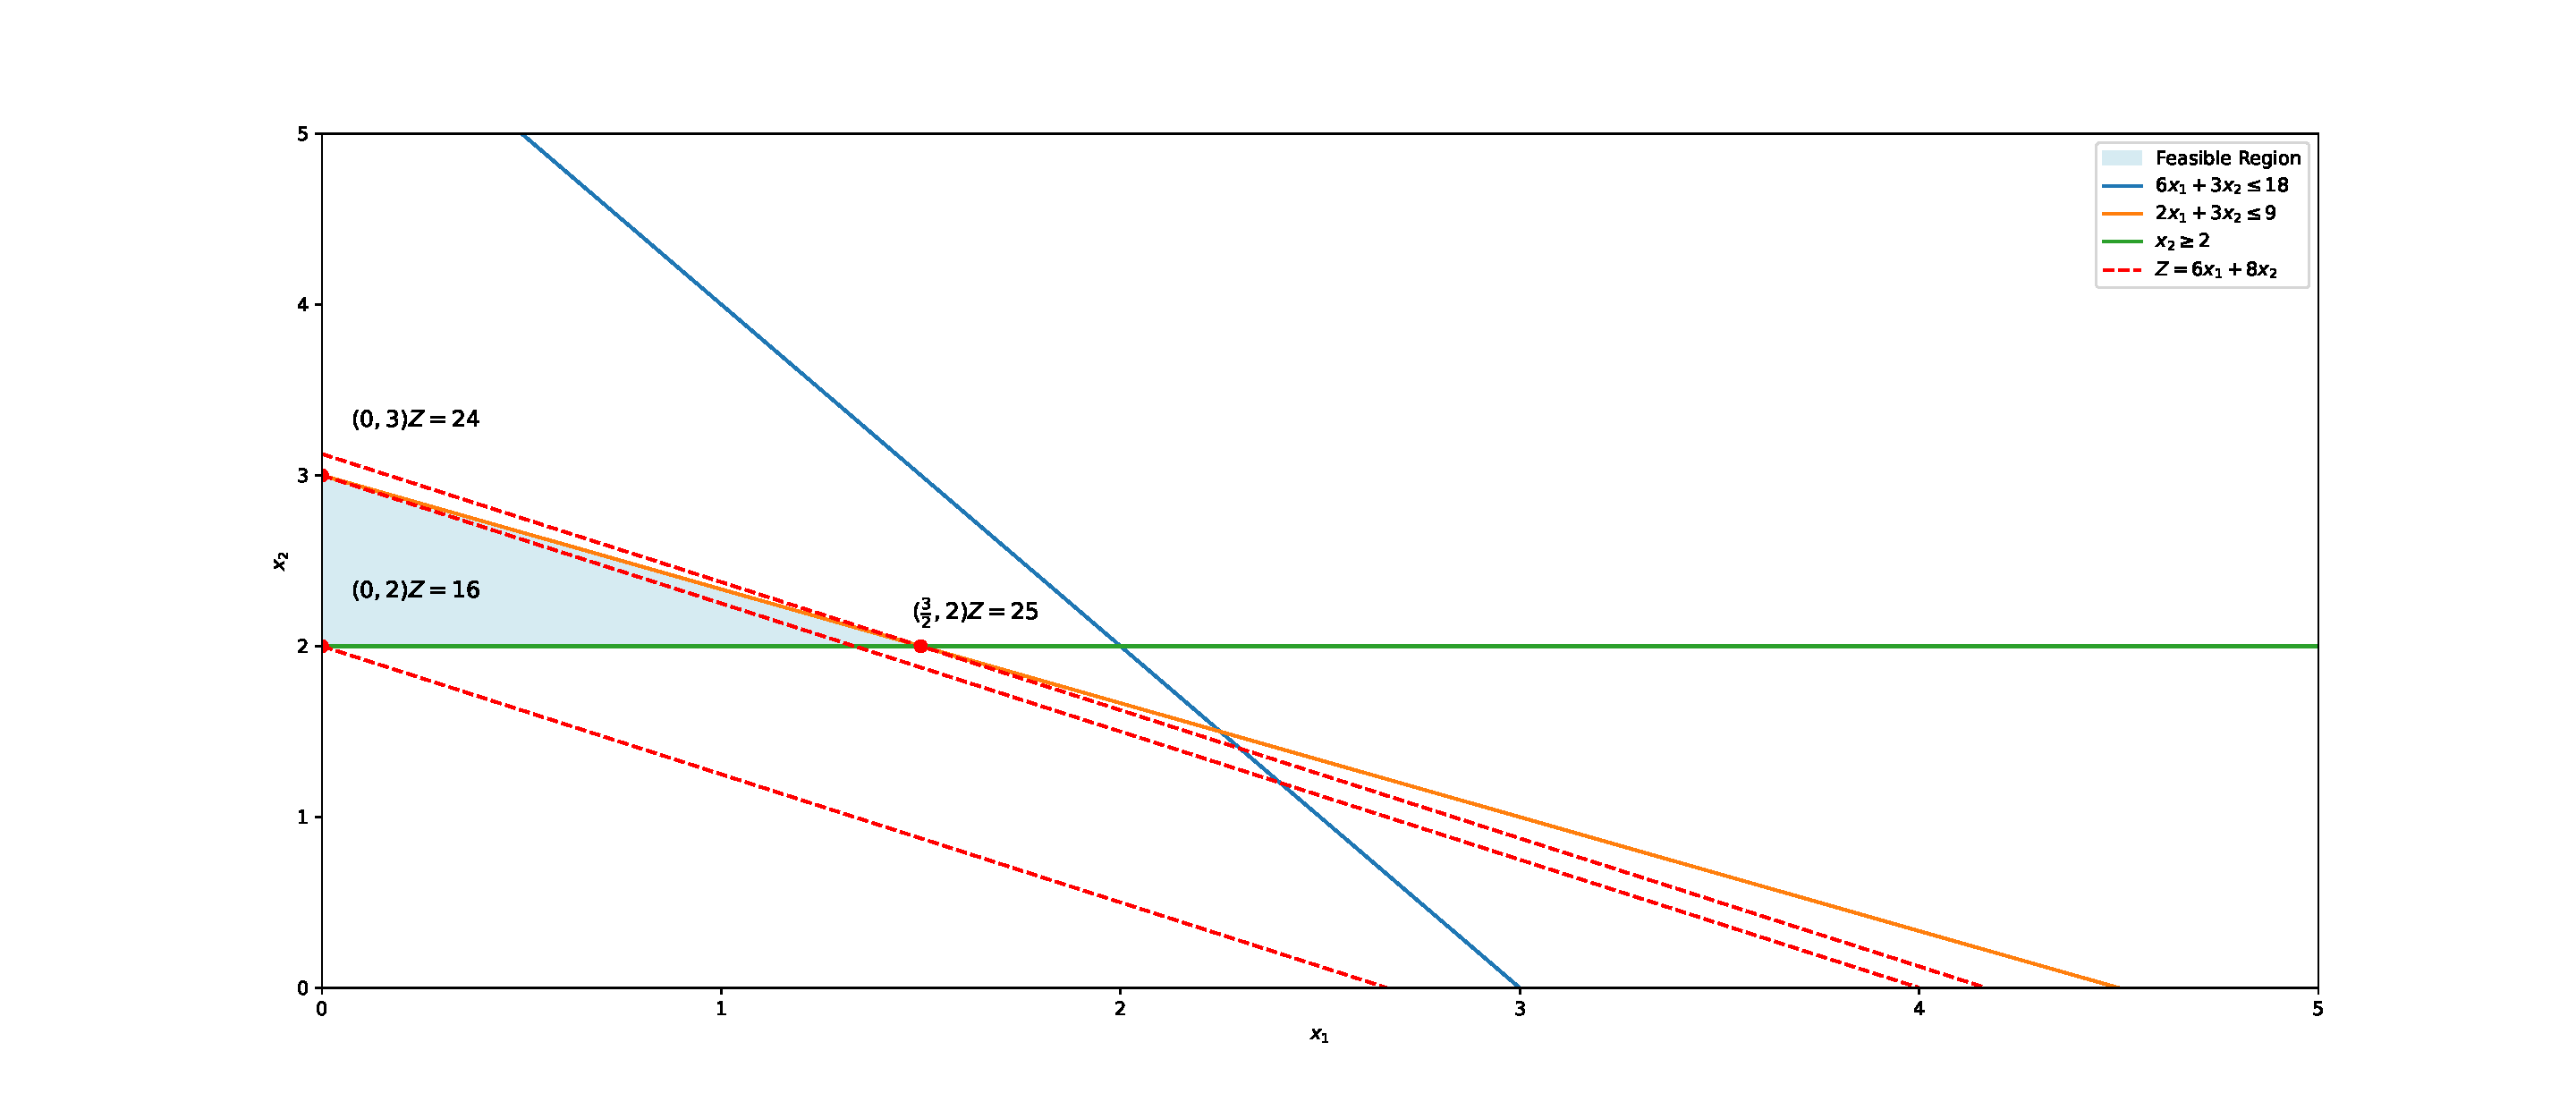
\includegraphics[width = \textwidth]{Exercice/PY/EX1/ex1.5.pdf}
\end{center}
\begin{center}
    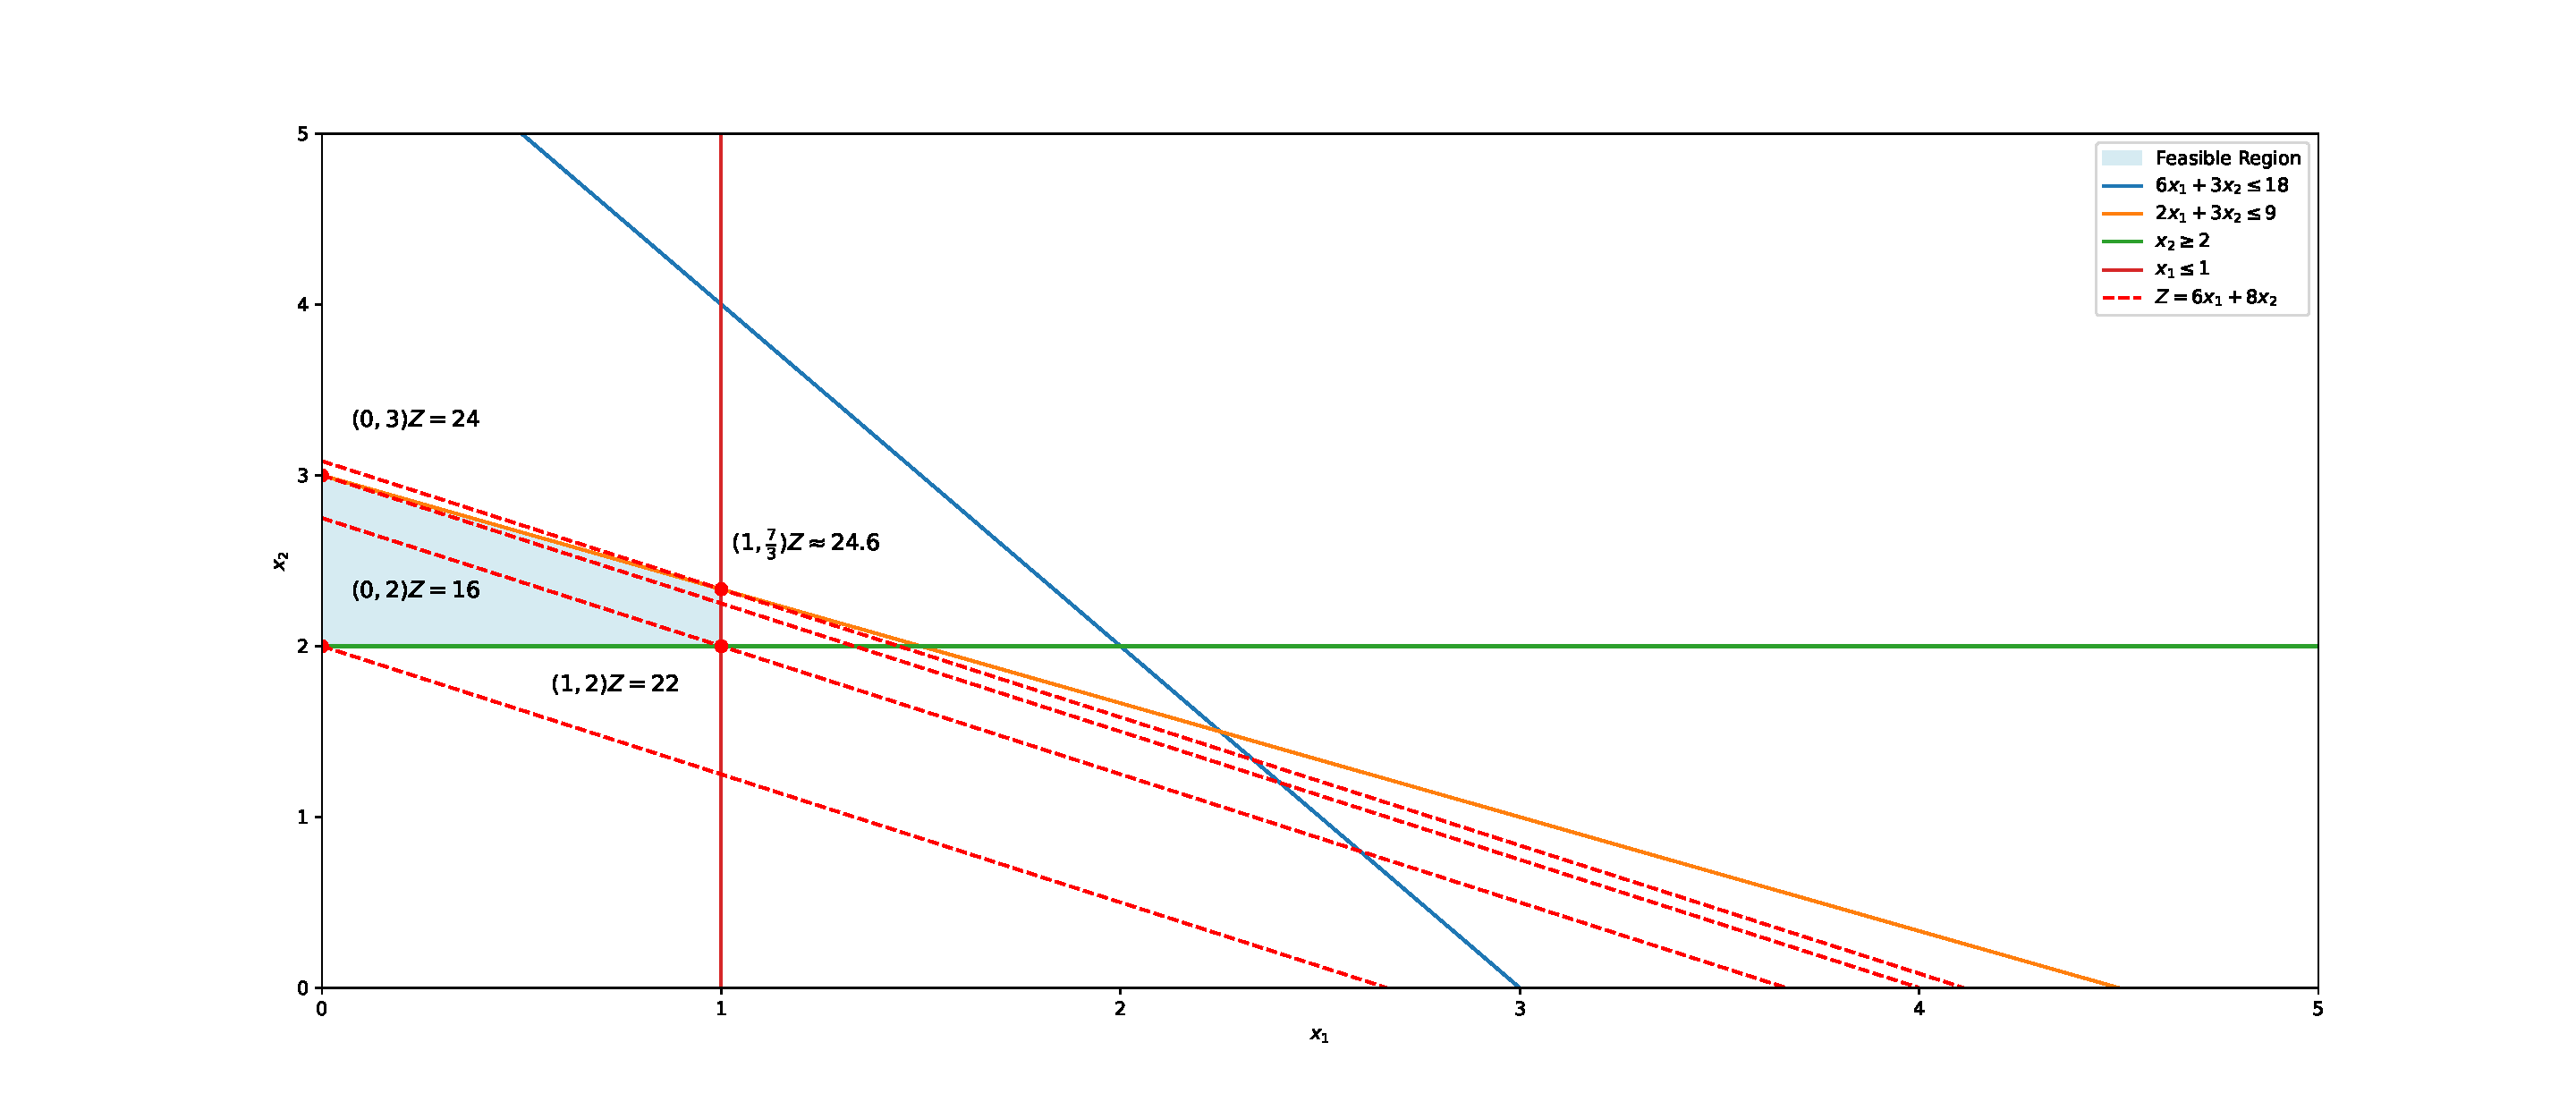
\includegraphics[width = \textwidth]{Exercice/PY/EX1/ex1.6.pdf}
\end{center}
\begin{center}
    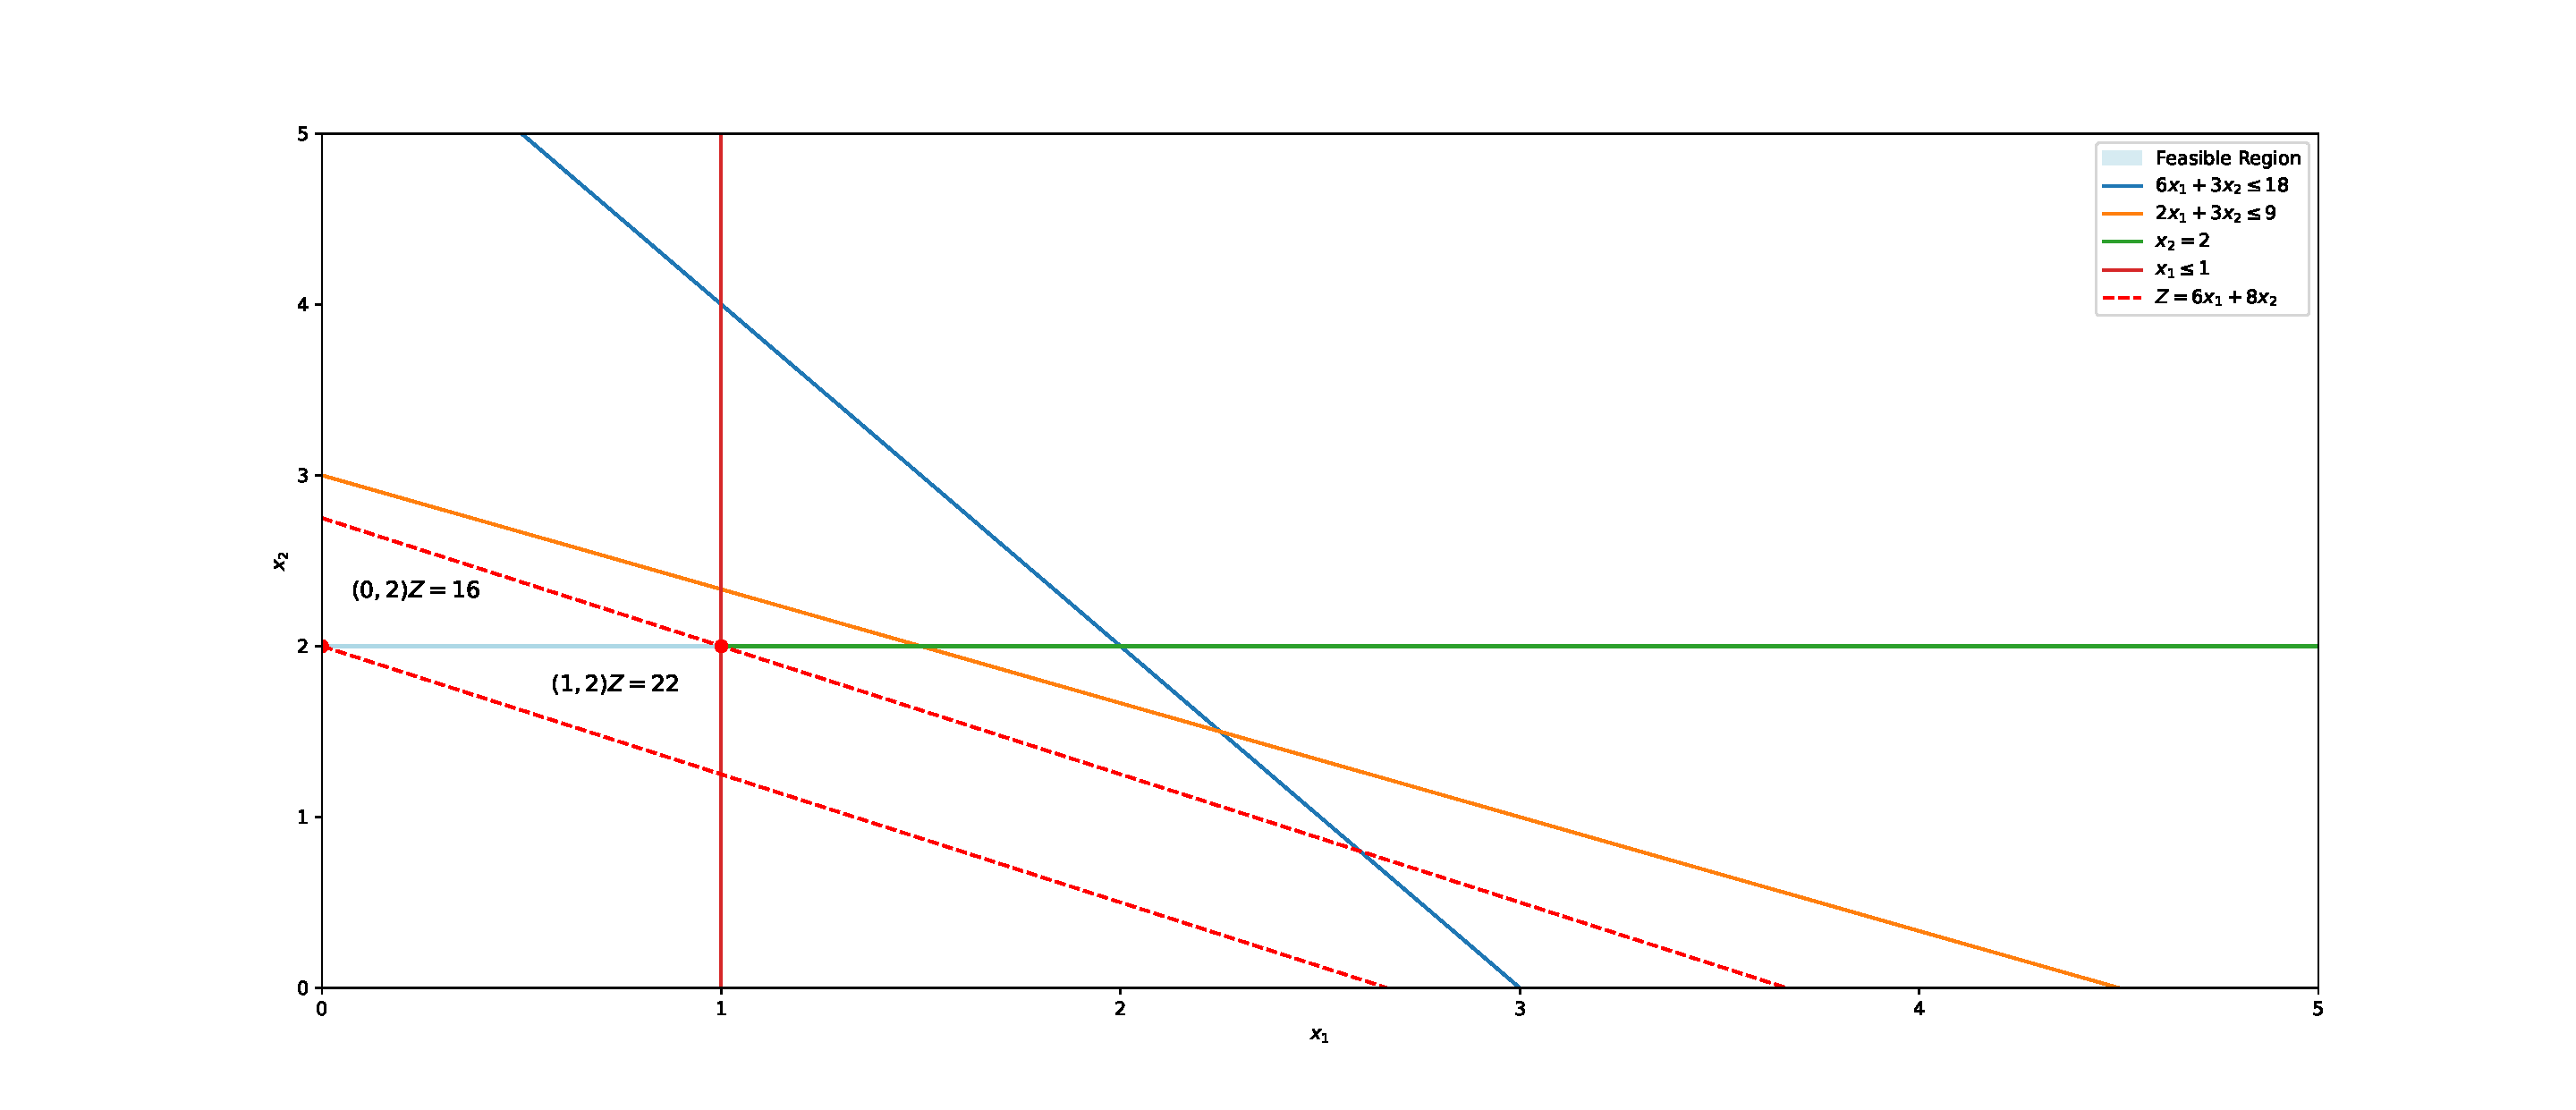
\includegraphics[width = \textwidth]{Exercice/PY/EX1/ex1.7.pdf}
\end{center}
\begin{center}
    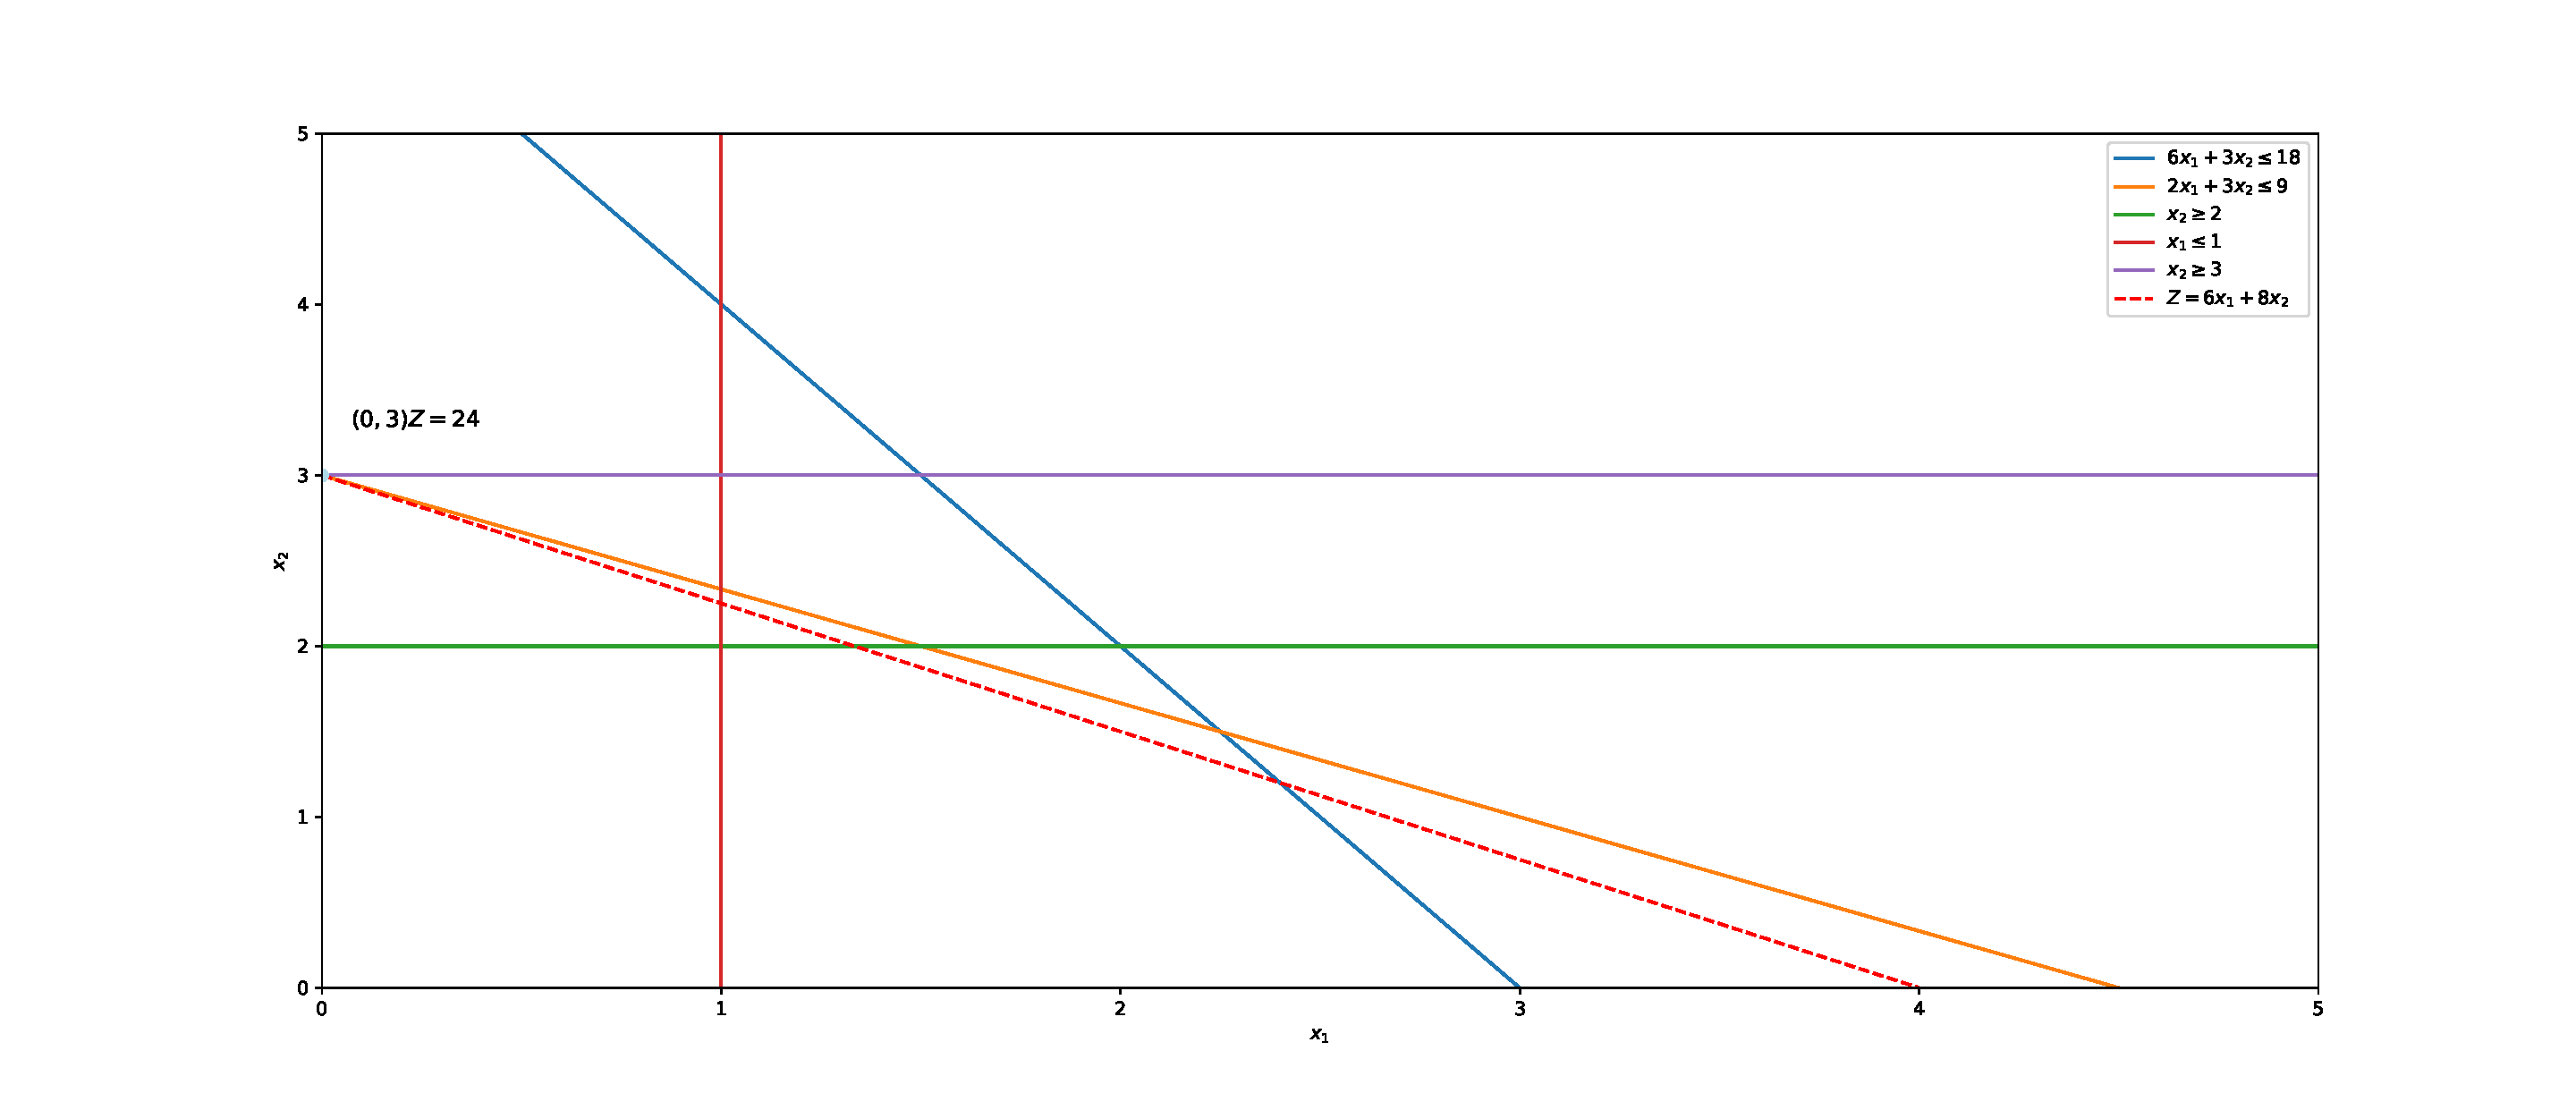
\includegraphics[width = \textwidth]{Exercice/PY/EX1/ex1.8.pdf}
\end{center}
\begin{center}
    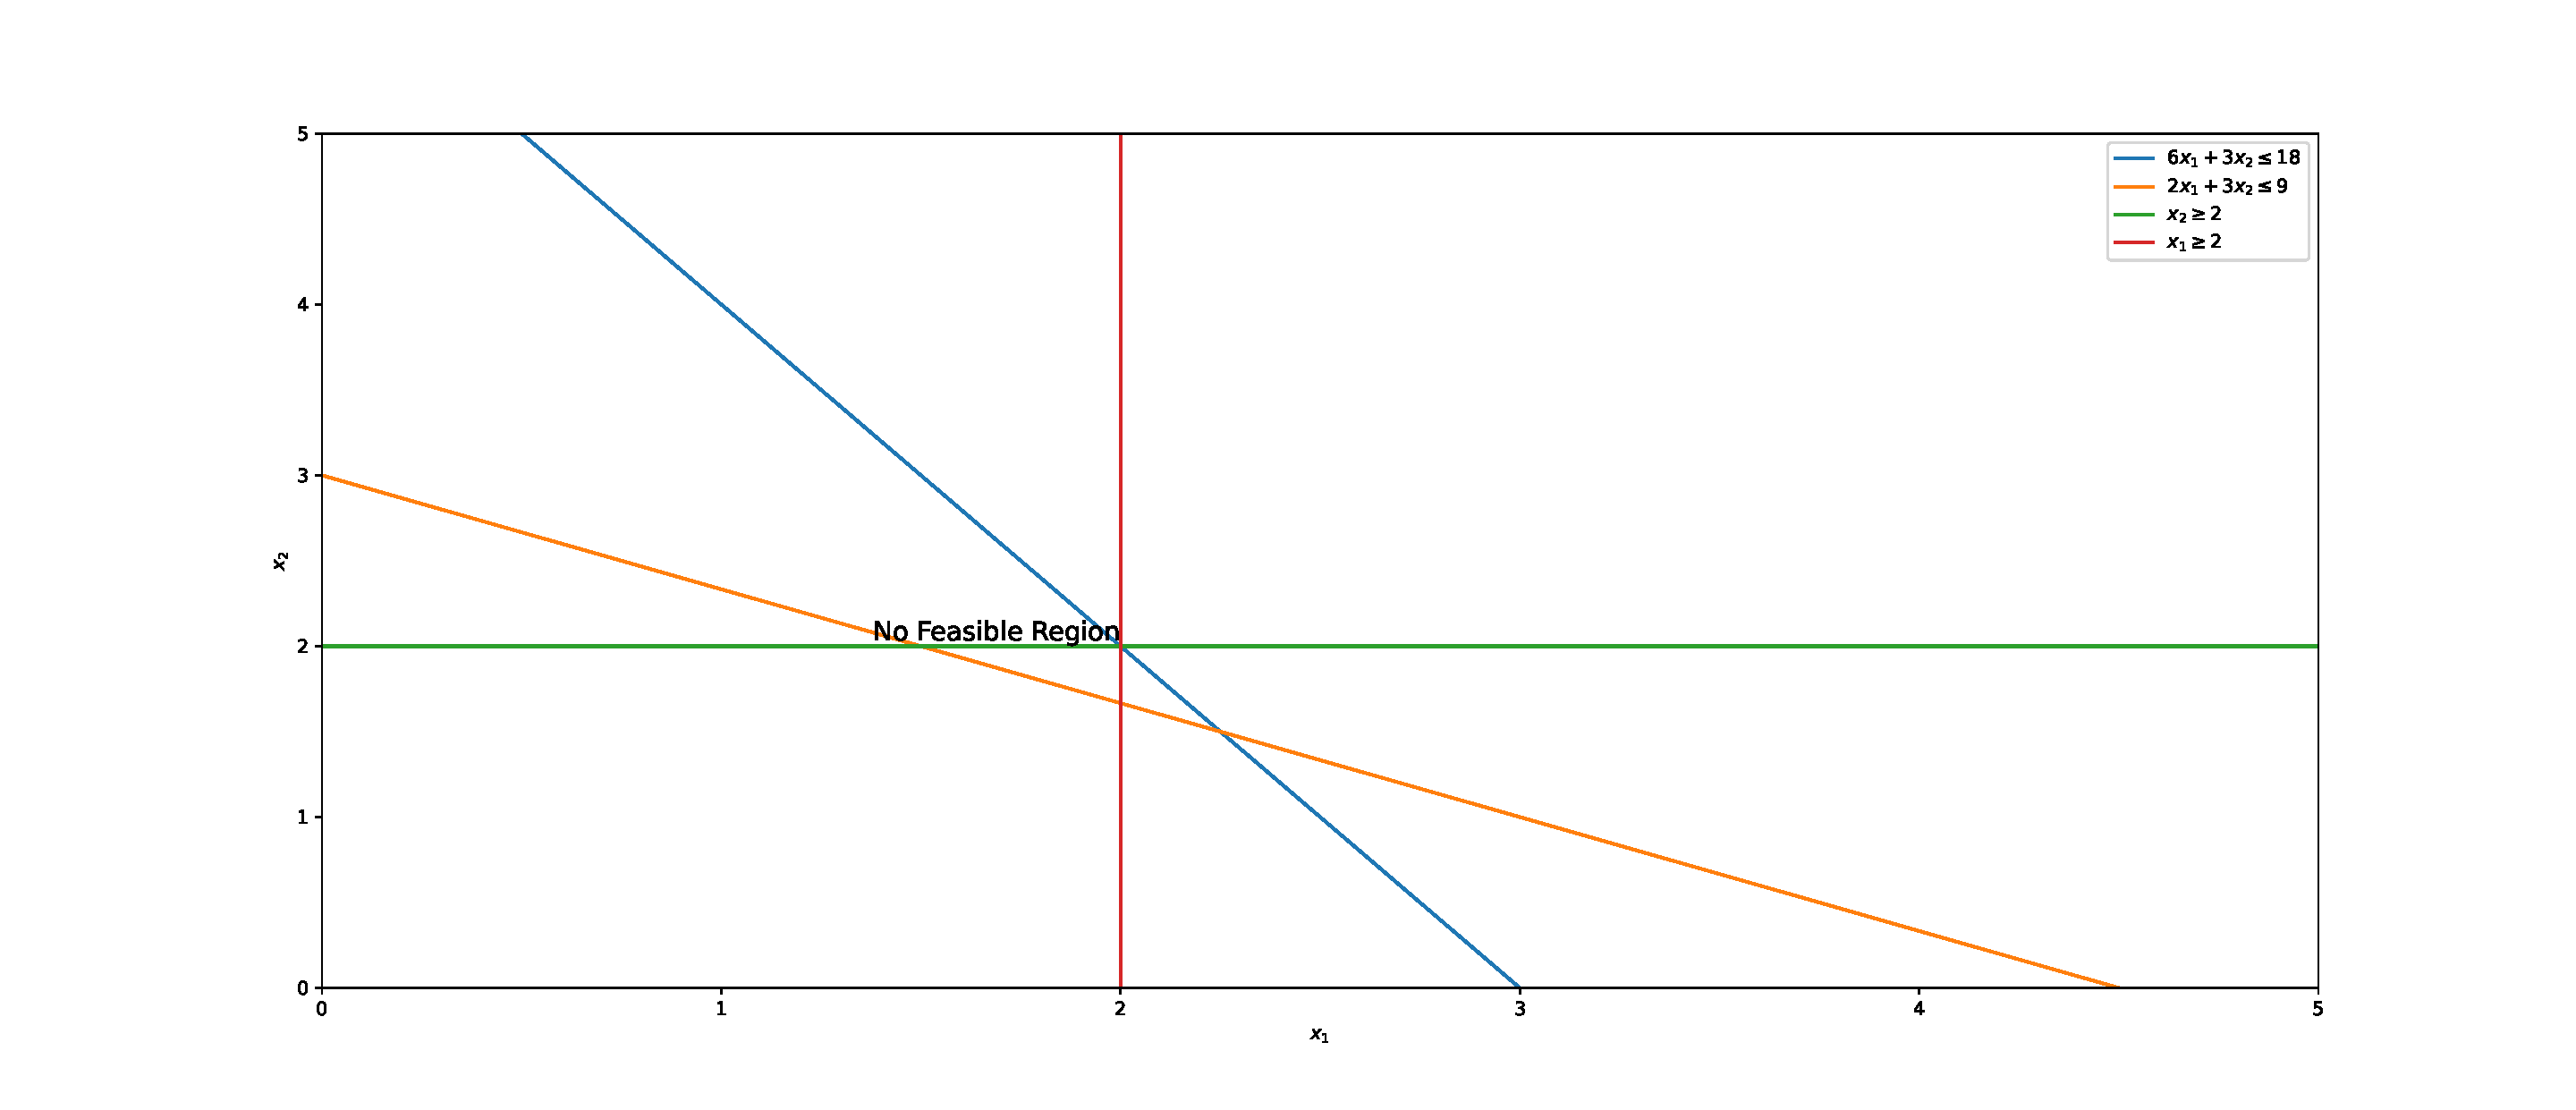
\includegraphics[width = \textwidth]{Exercice/PY/EX1/ex1.9.pdf}
\end{center}




\newpage
\[ \text{min } Z = x_1 - 2x_2 \quad \Longrightarrow \quad \text{max } -Z = - x_1 + 2x_2 \]  

\[    
\left\{
    \begin{array}{l}
        6x_{1} + 3x_{2} \leq 18 \\[2pt]
        2x_{1} + 3x_{2} \leq 9 \\[2pt]
        x_{1}, x_{2} \text{ are integers}
    \end{array}
    \right.
\]

\begin{center}
    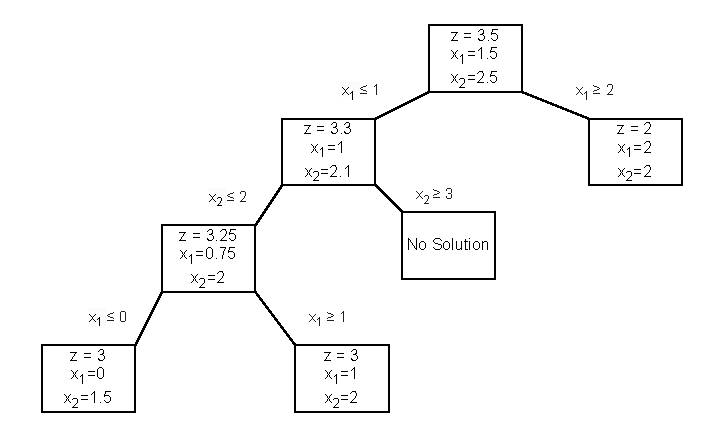
\includegraphics{Exercice/PY/EX2/b2.drawio.pdf}
\end{center}

\vspace{0.5cm}

\[\text{Optimal Solution is }\hspace{0.1cm} \boxed{(x_1,x_2) = (1,2)}\]


\vspace{0.5cm}

\begin{prettyBox}{Note}{red}
We did not branch the node (\(Z = 3, x_1 = 0, x_2 = 1.5\)) because another node 
at the same level (\(Z = 3, x_1 = 1, x_2 = 2\)) was already completed. Continuing 
to branch the first node would only cause \(Z\) to keep decreasing. Hence, we pruned it.
\end{prettyBox}

\begin{center}
    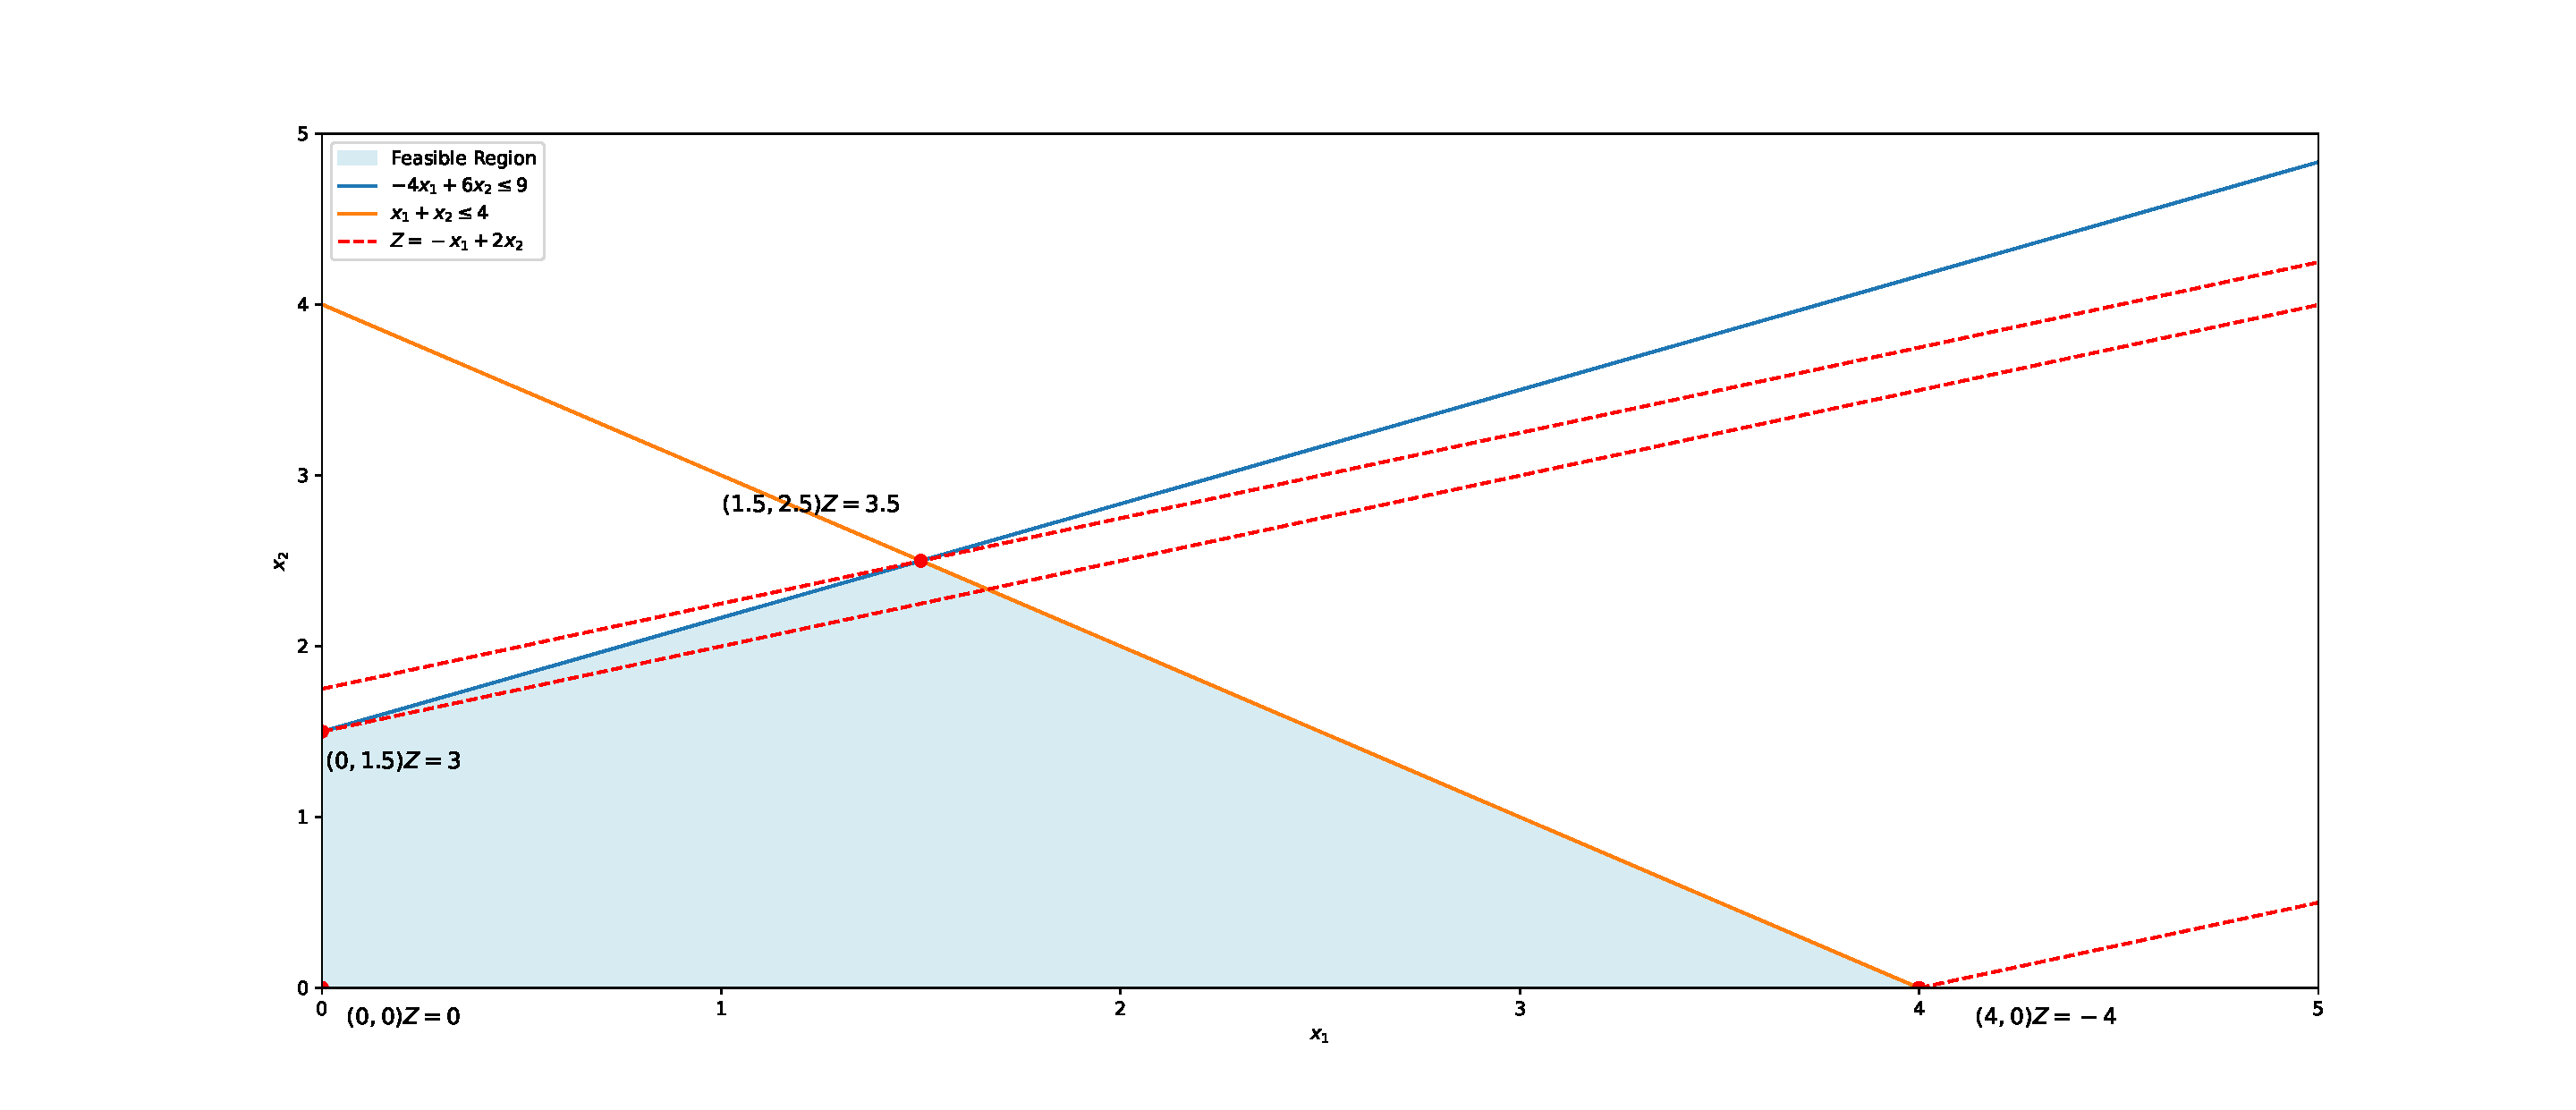
\includegraphics[width = \textwidth]{Exercice/PY/EX2/ex2.1.pdf}
\end{center}


\begin{center}
    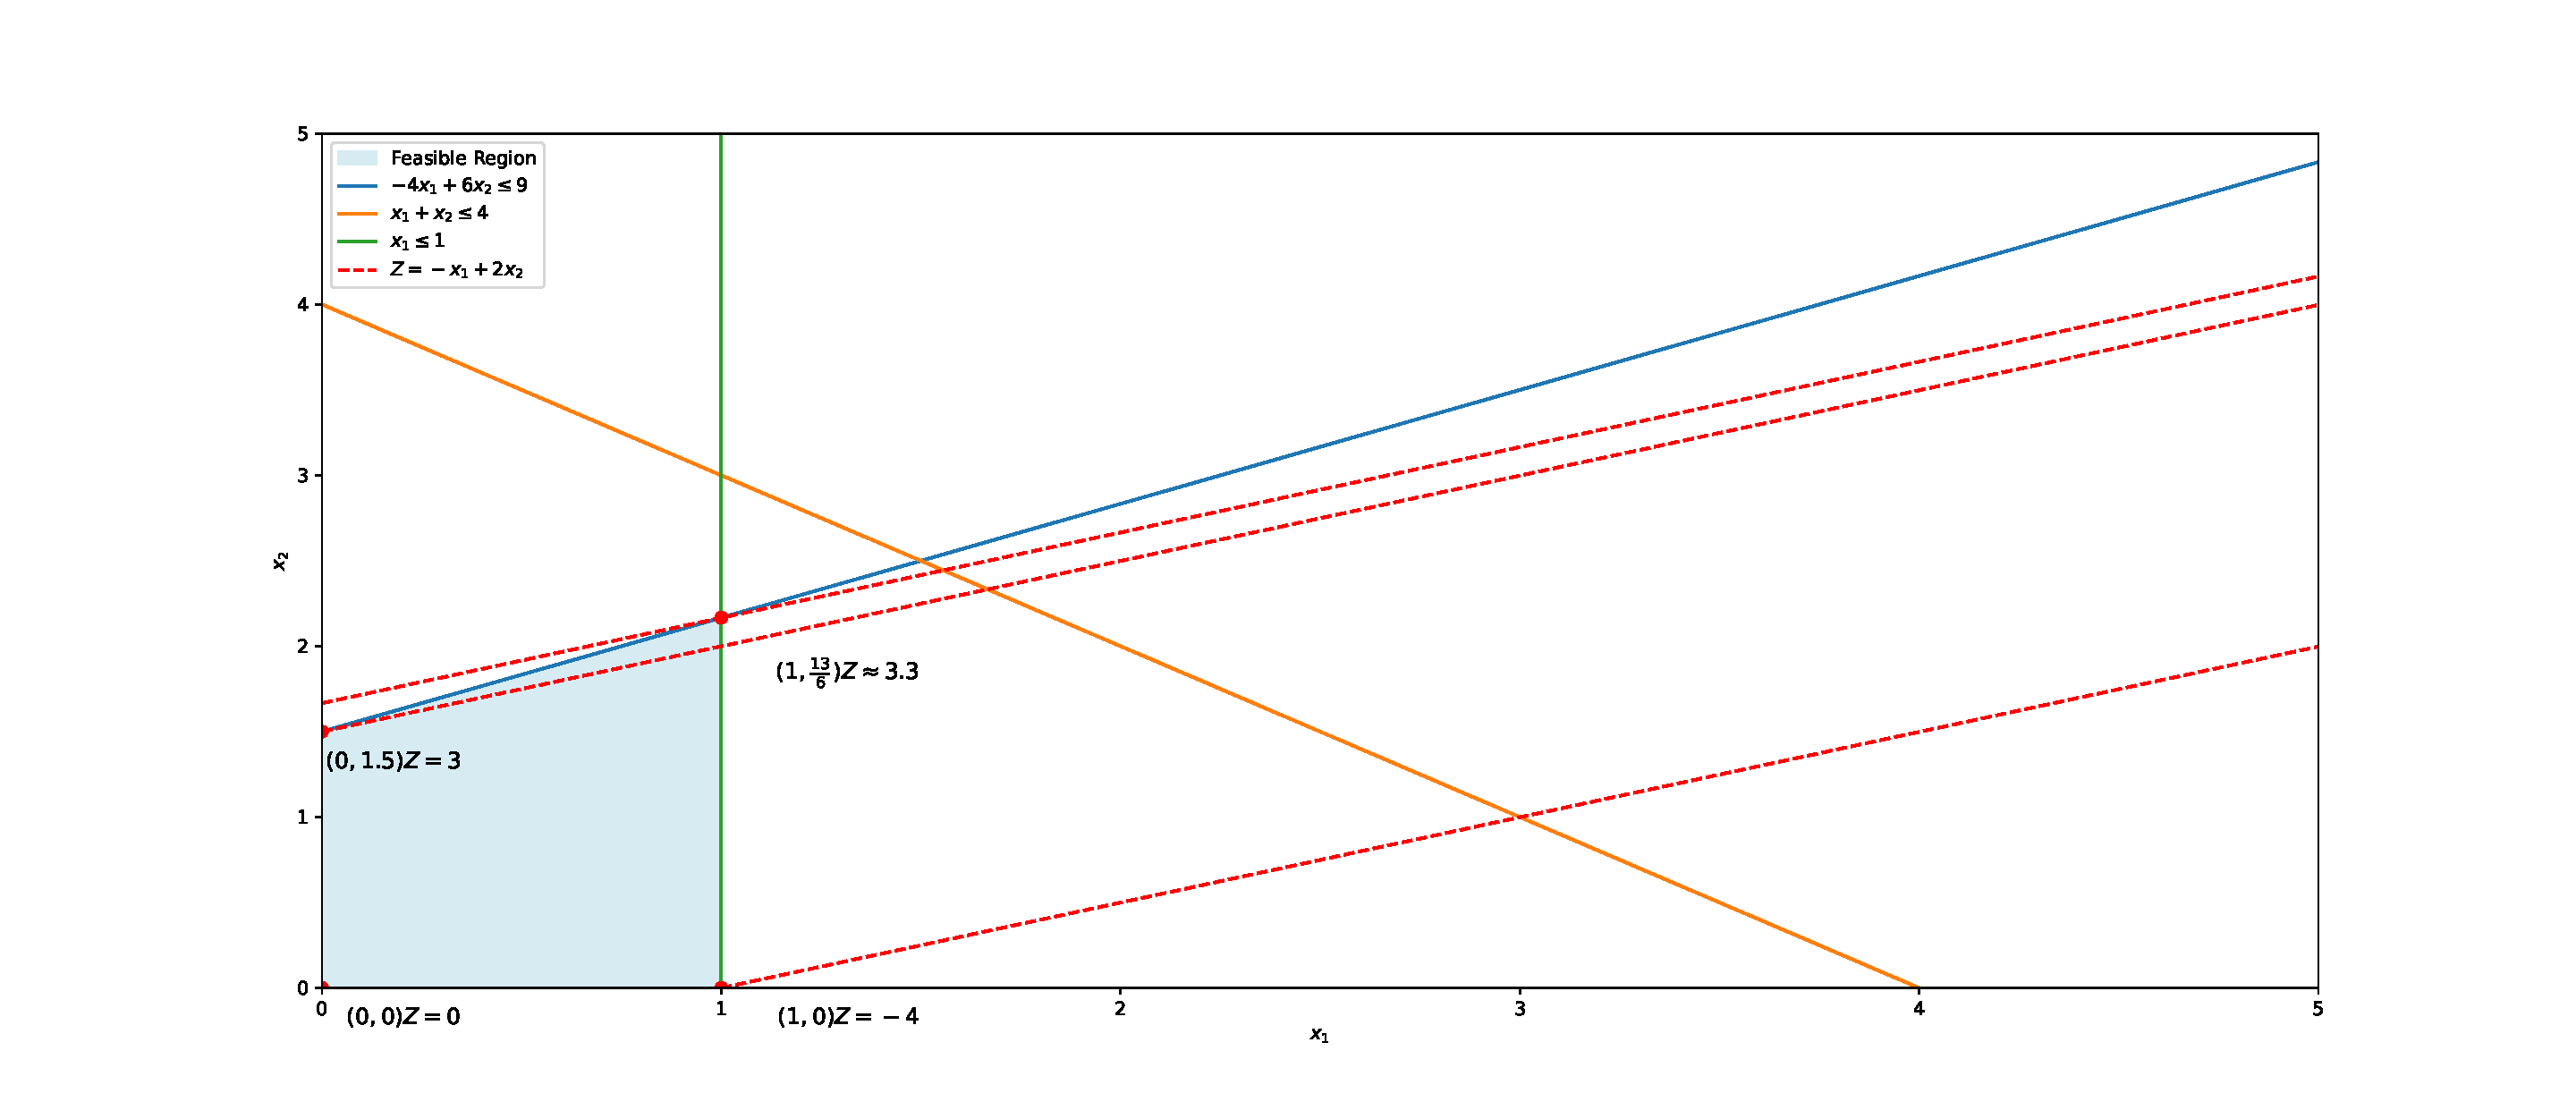
\includegraphics[width = \textwidth]{Exercice/PY/EX2/ex2.2.pdf}
\end{center}


\begin{center}
    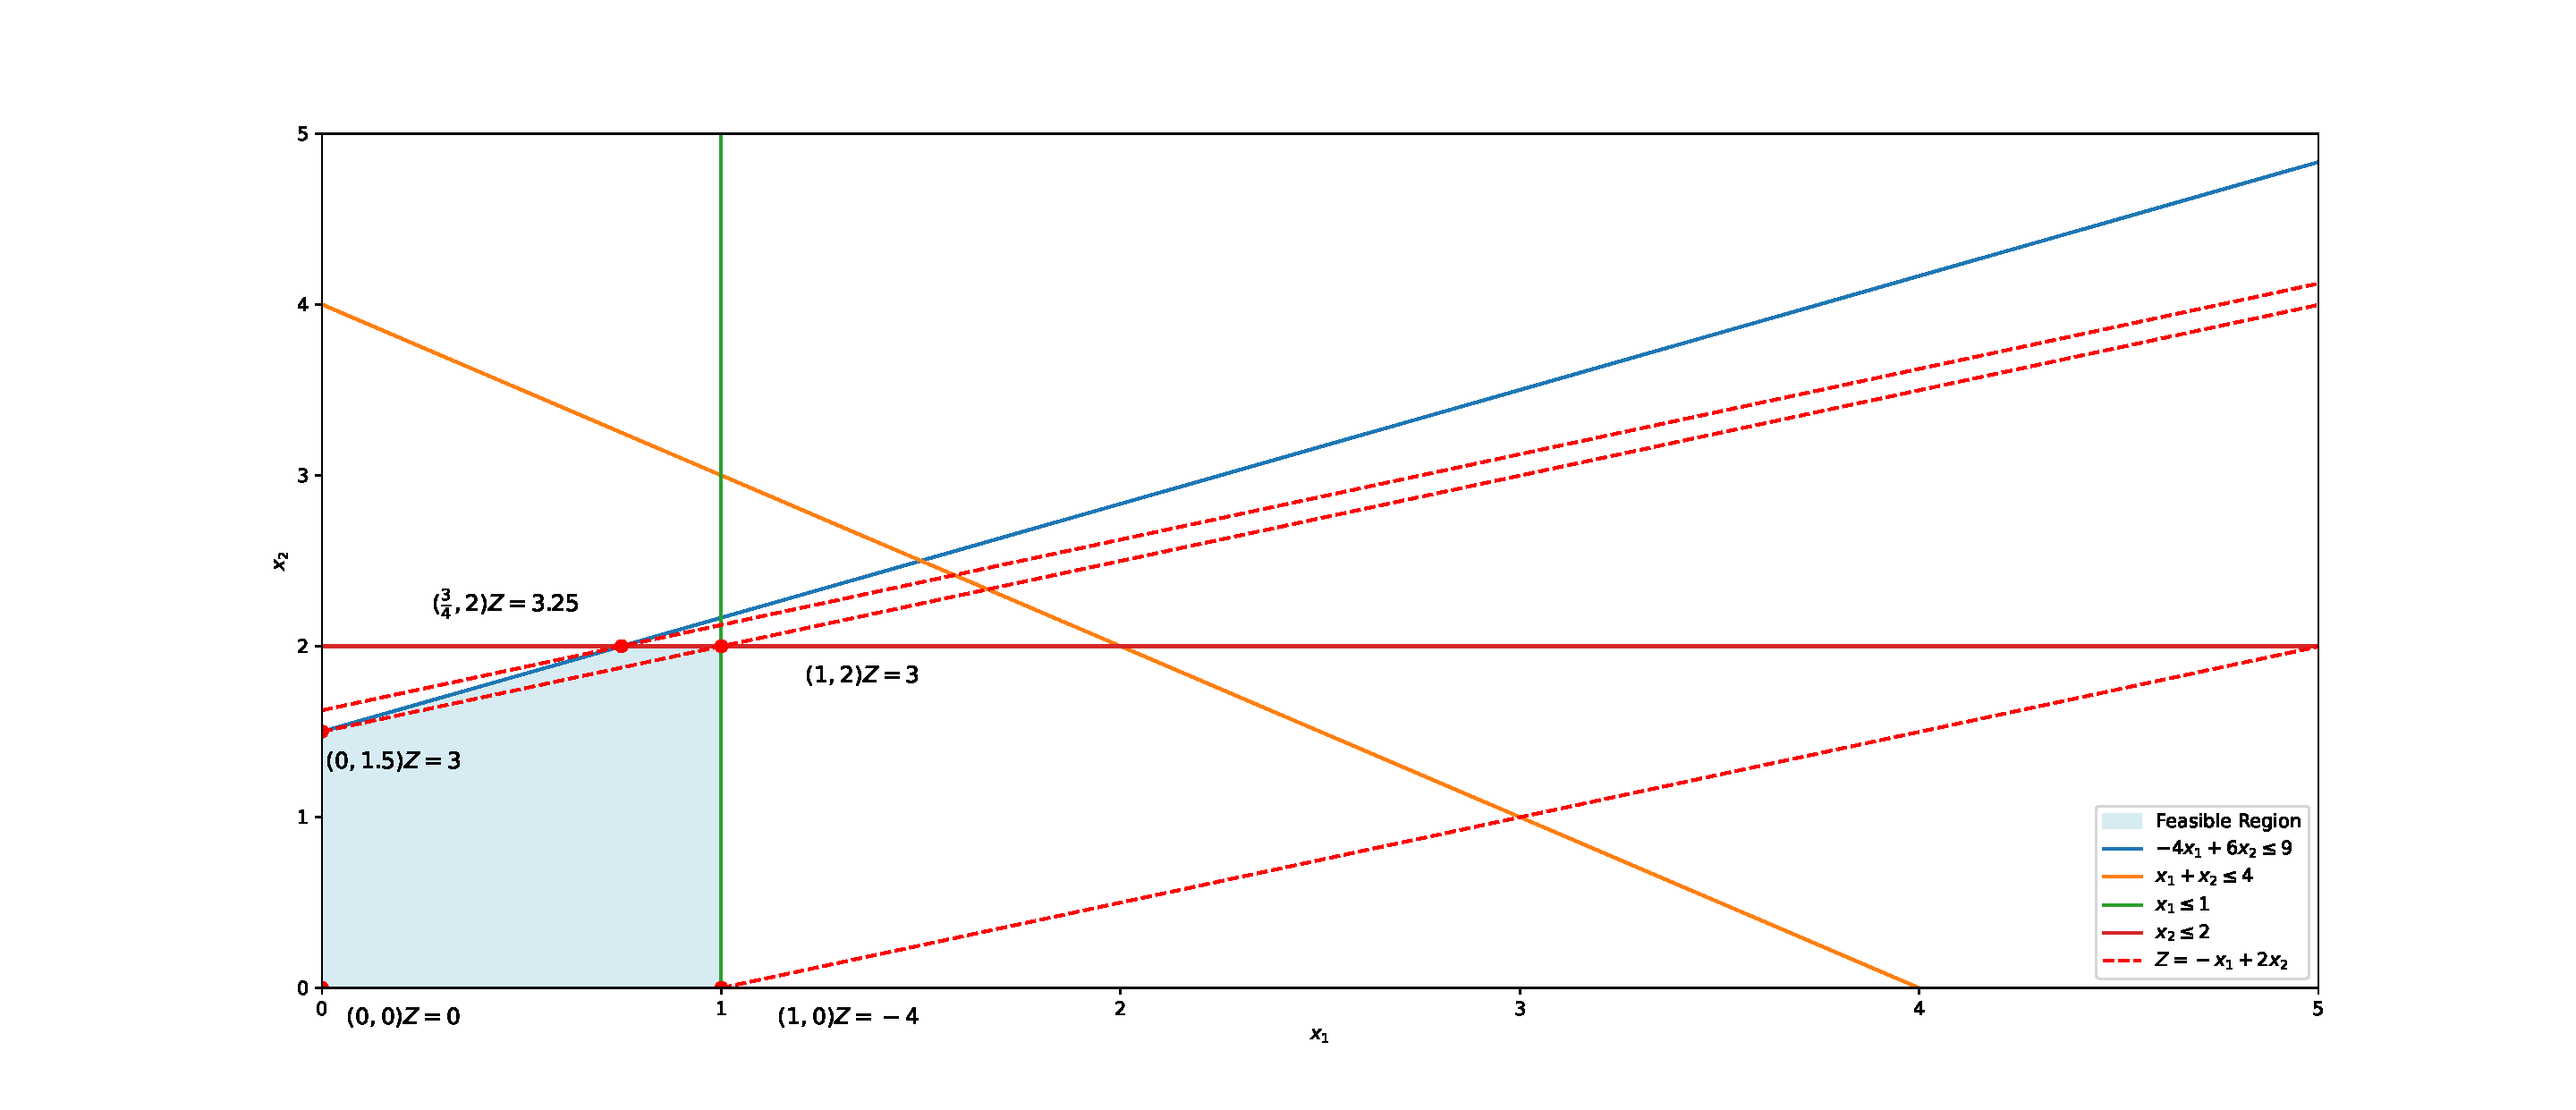
\includegraphics[width = \textwidth]{Exercice/PY/EX2/ex2.3.pdf}
\end{center}

\begin{center}
    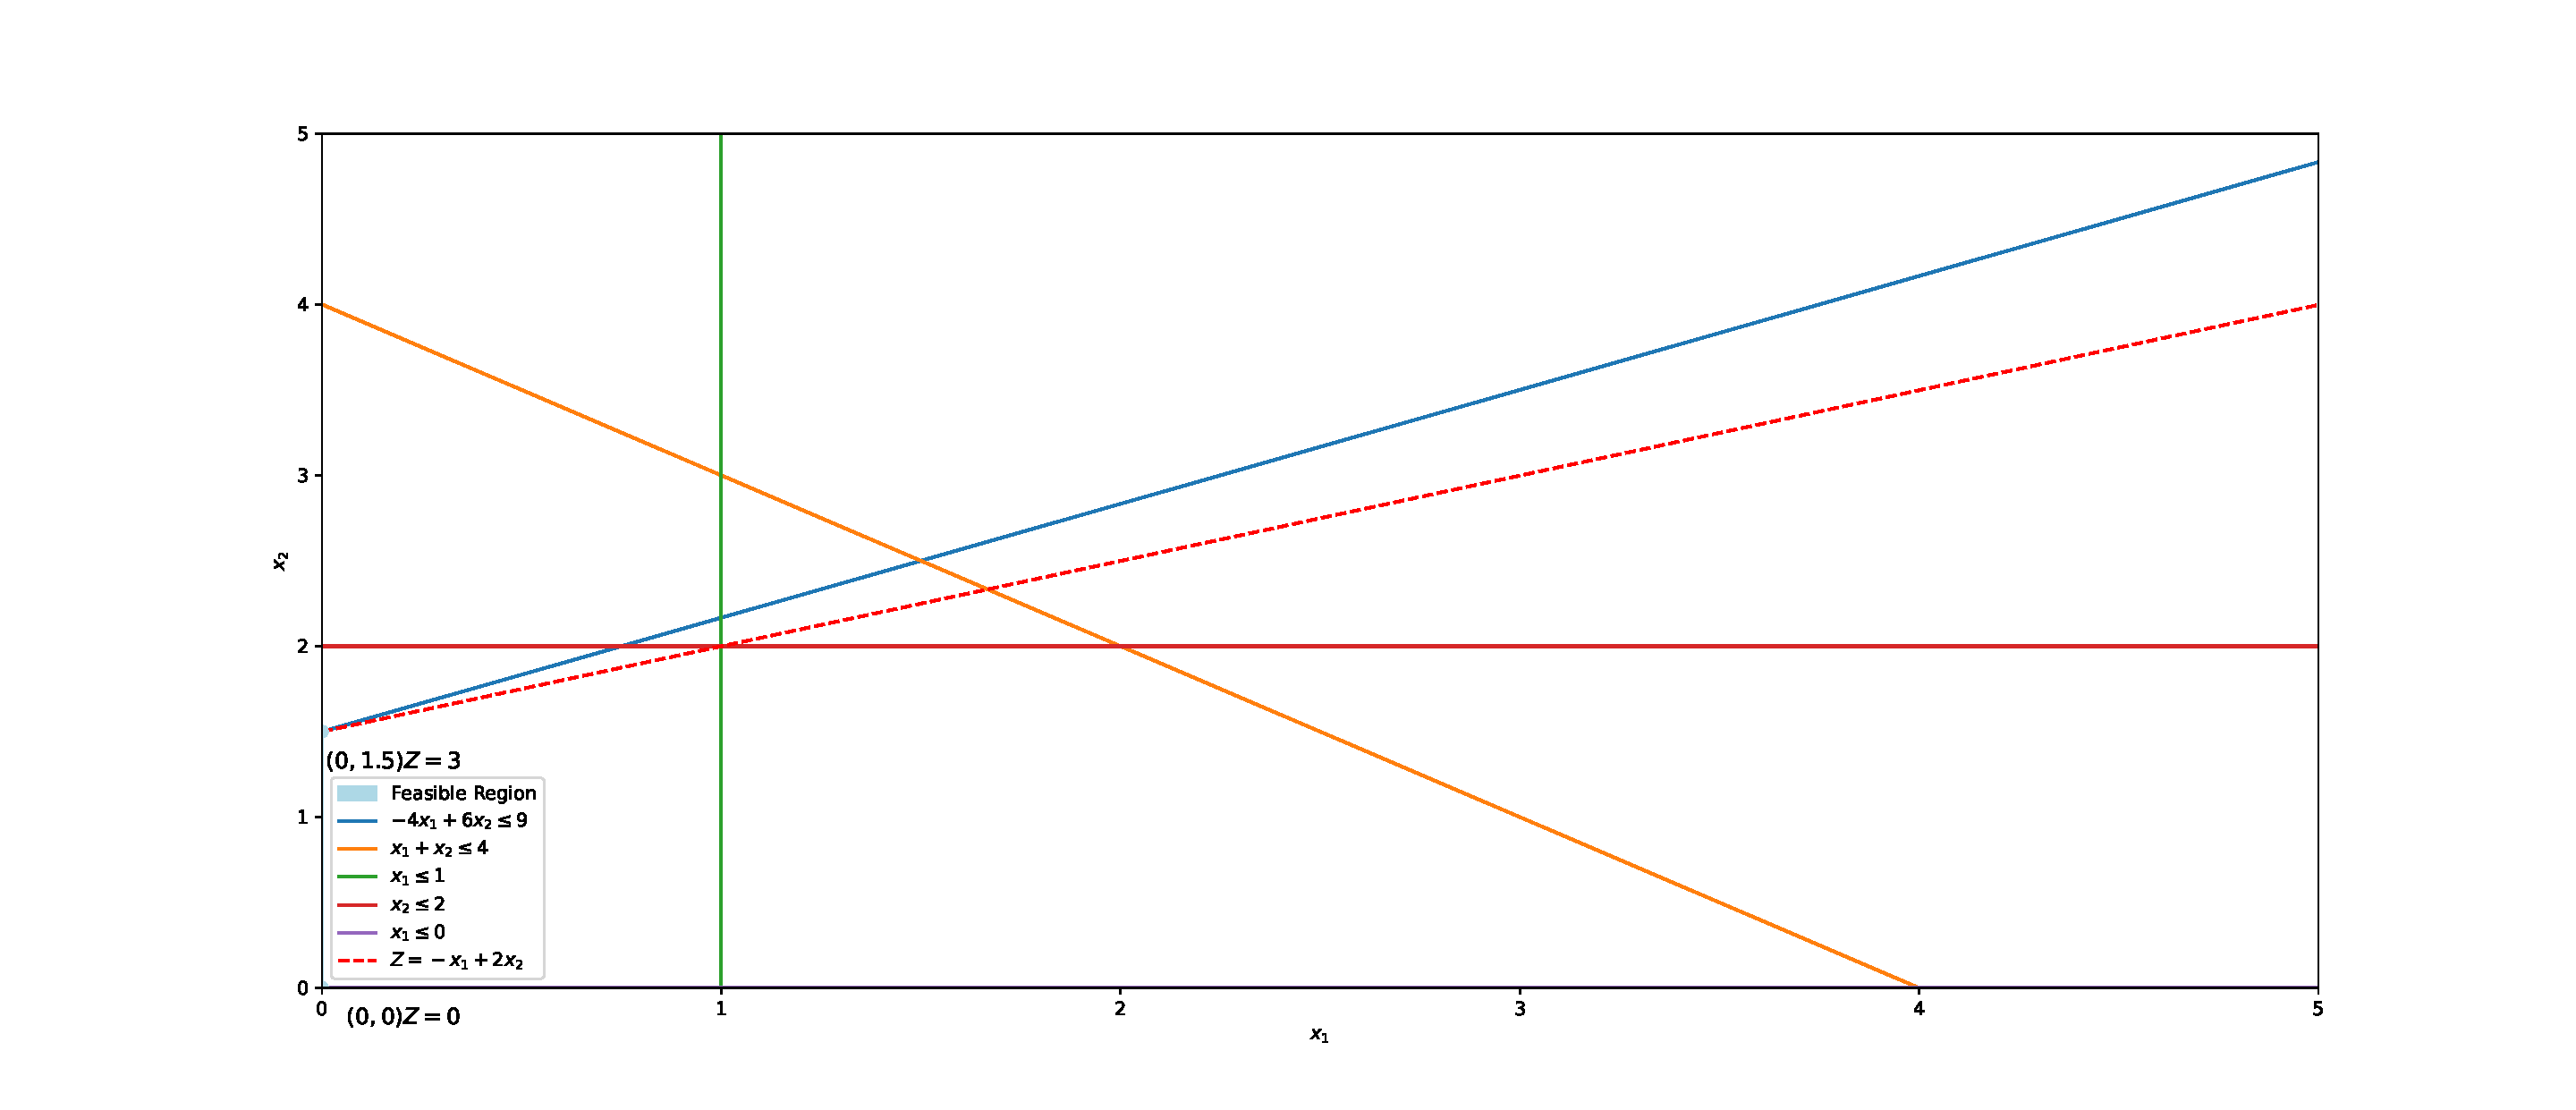
\includegraphics[width = \textwidth]{Exercice/PY/EX2/ex2.4.pdf}
\end{center}
\begin{center}
    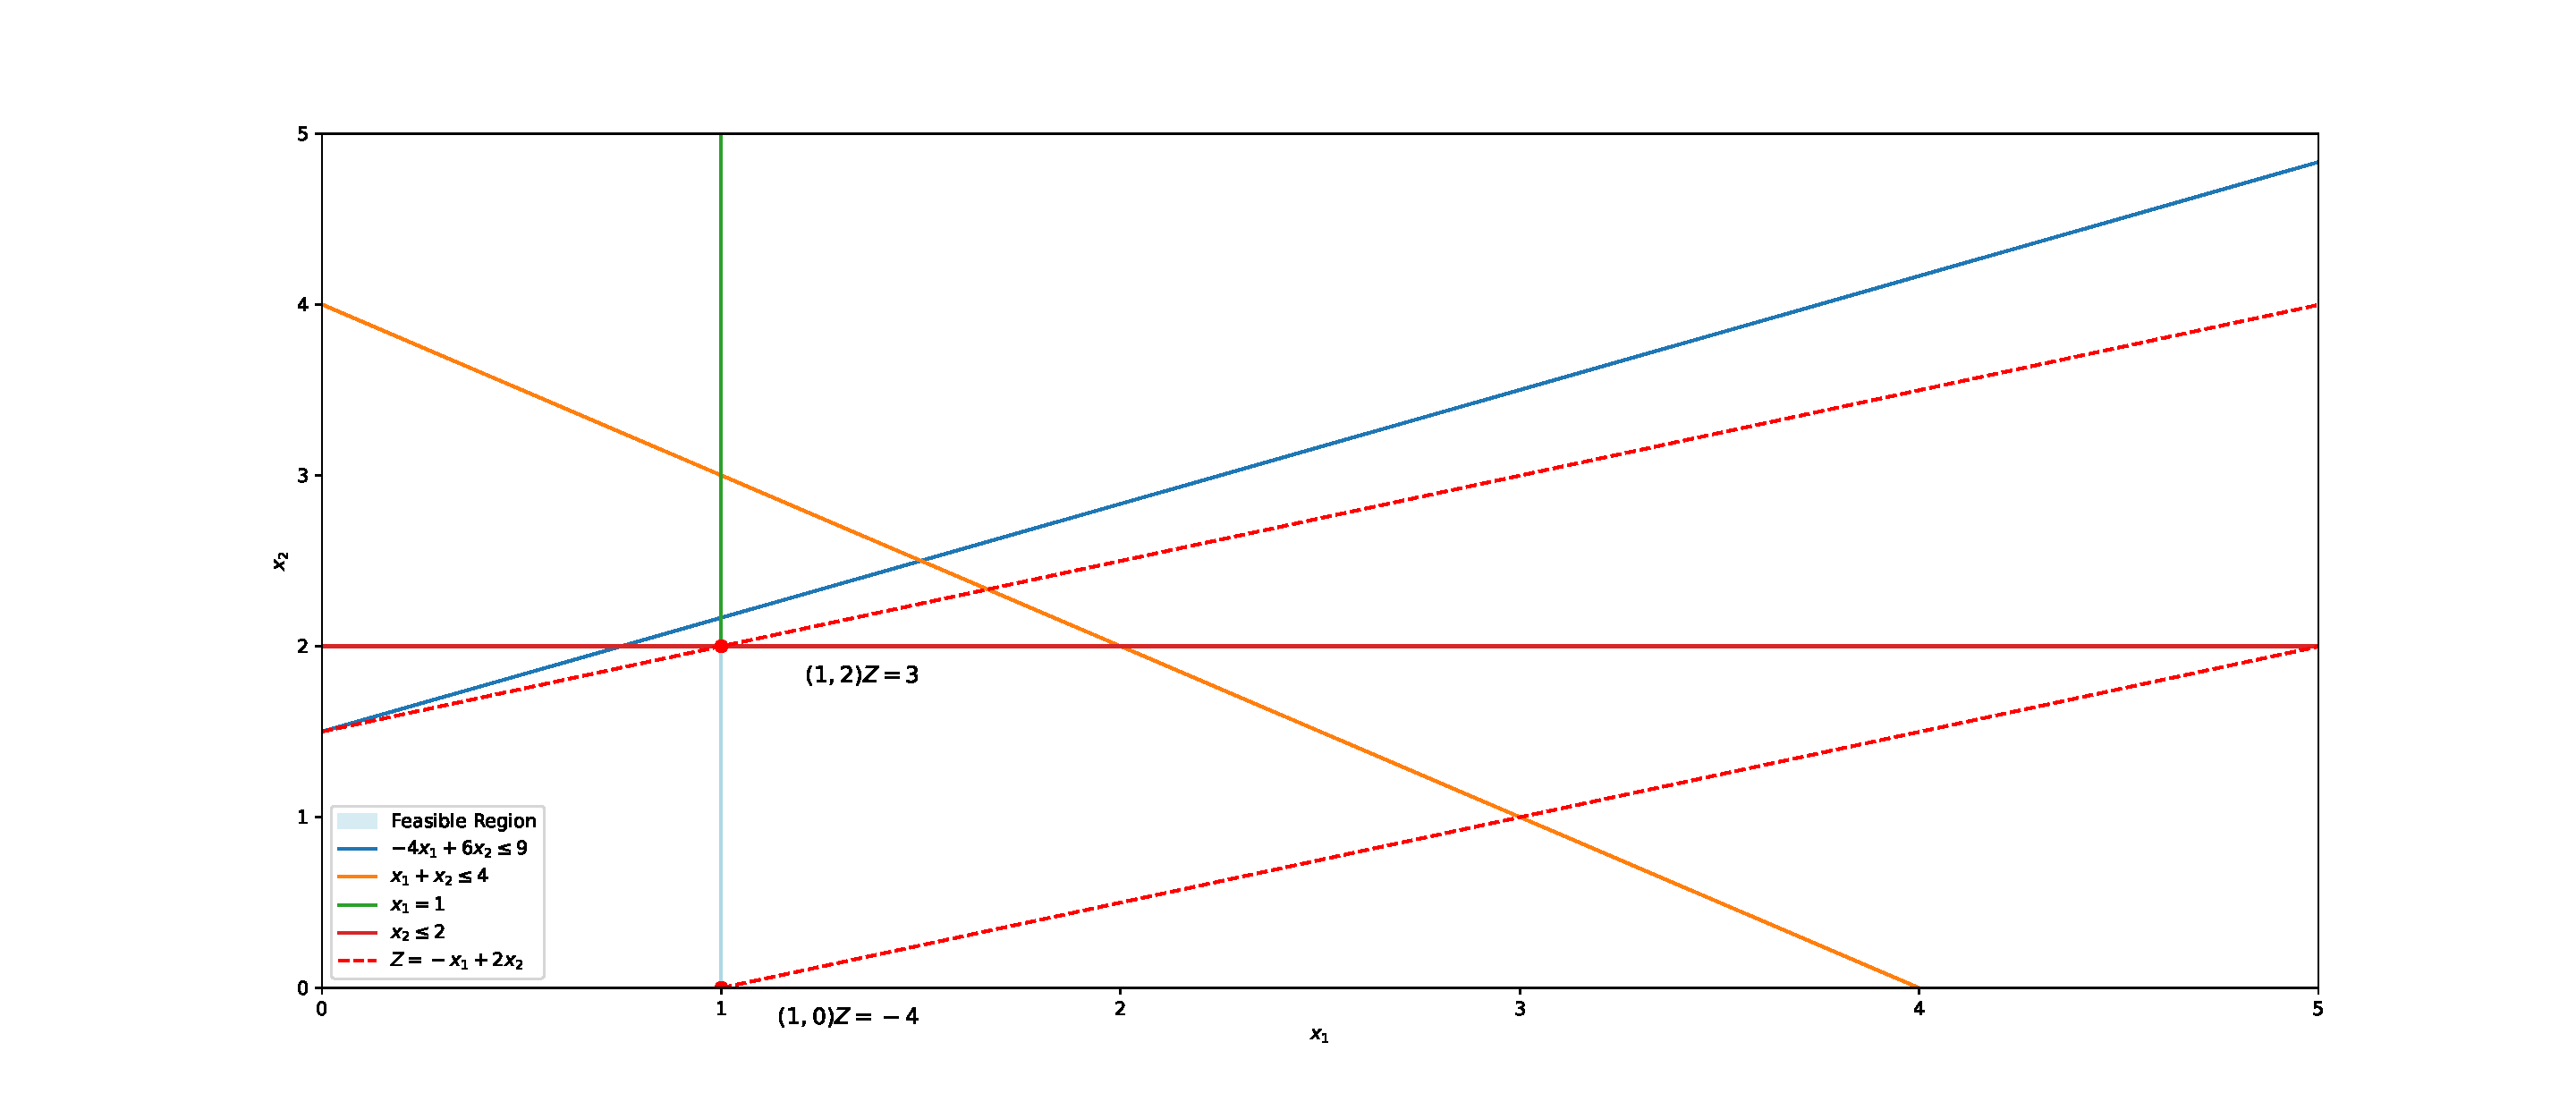
\includegraphics[width = \textwidth]{Exercice/PY/EX2/ex2.5.pdf}
\end{center}
\begin{center}
    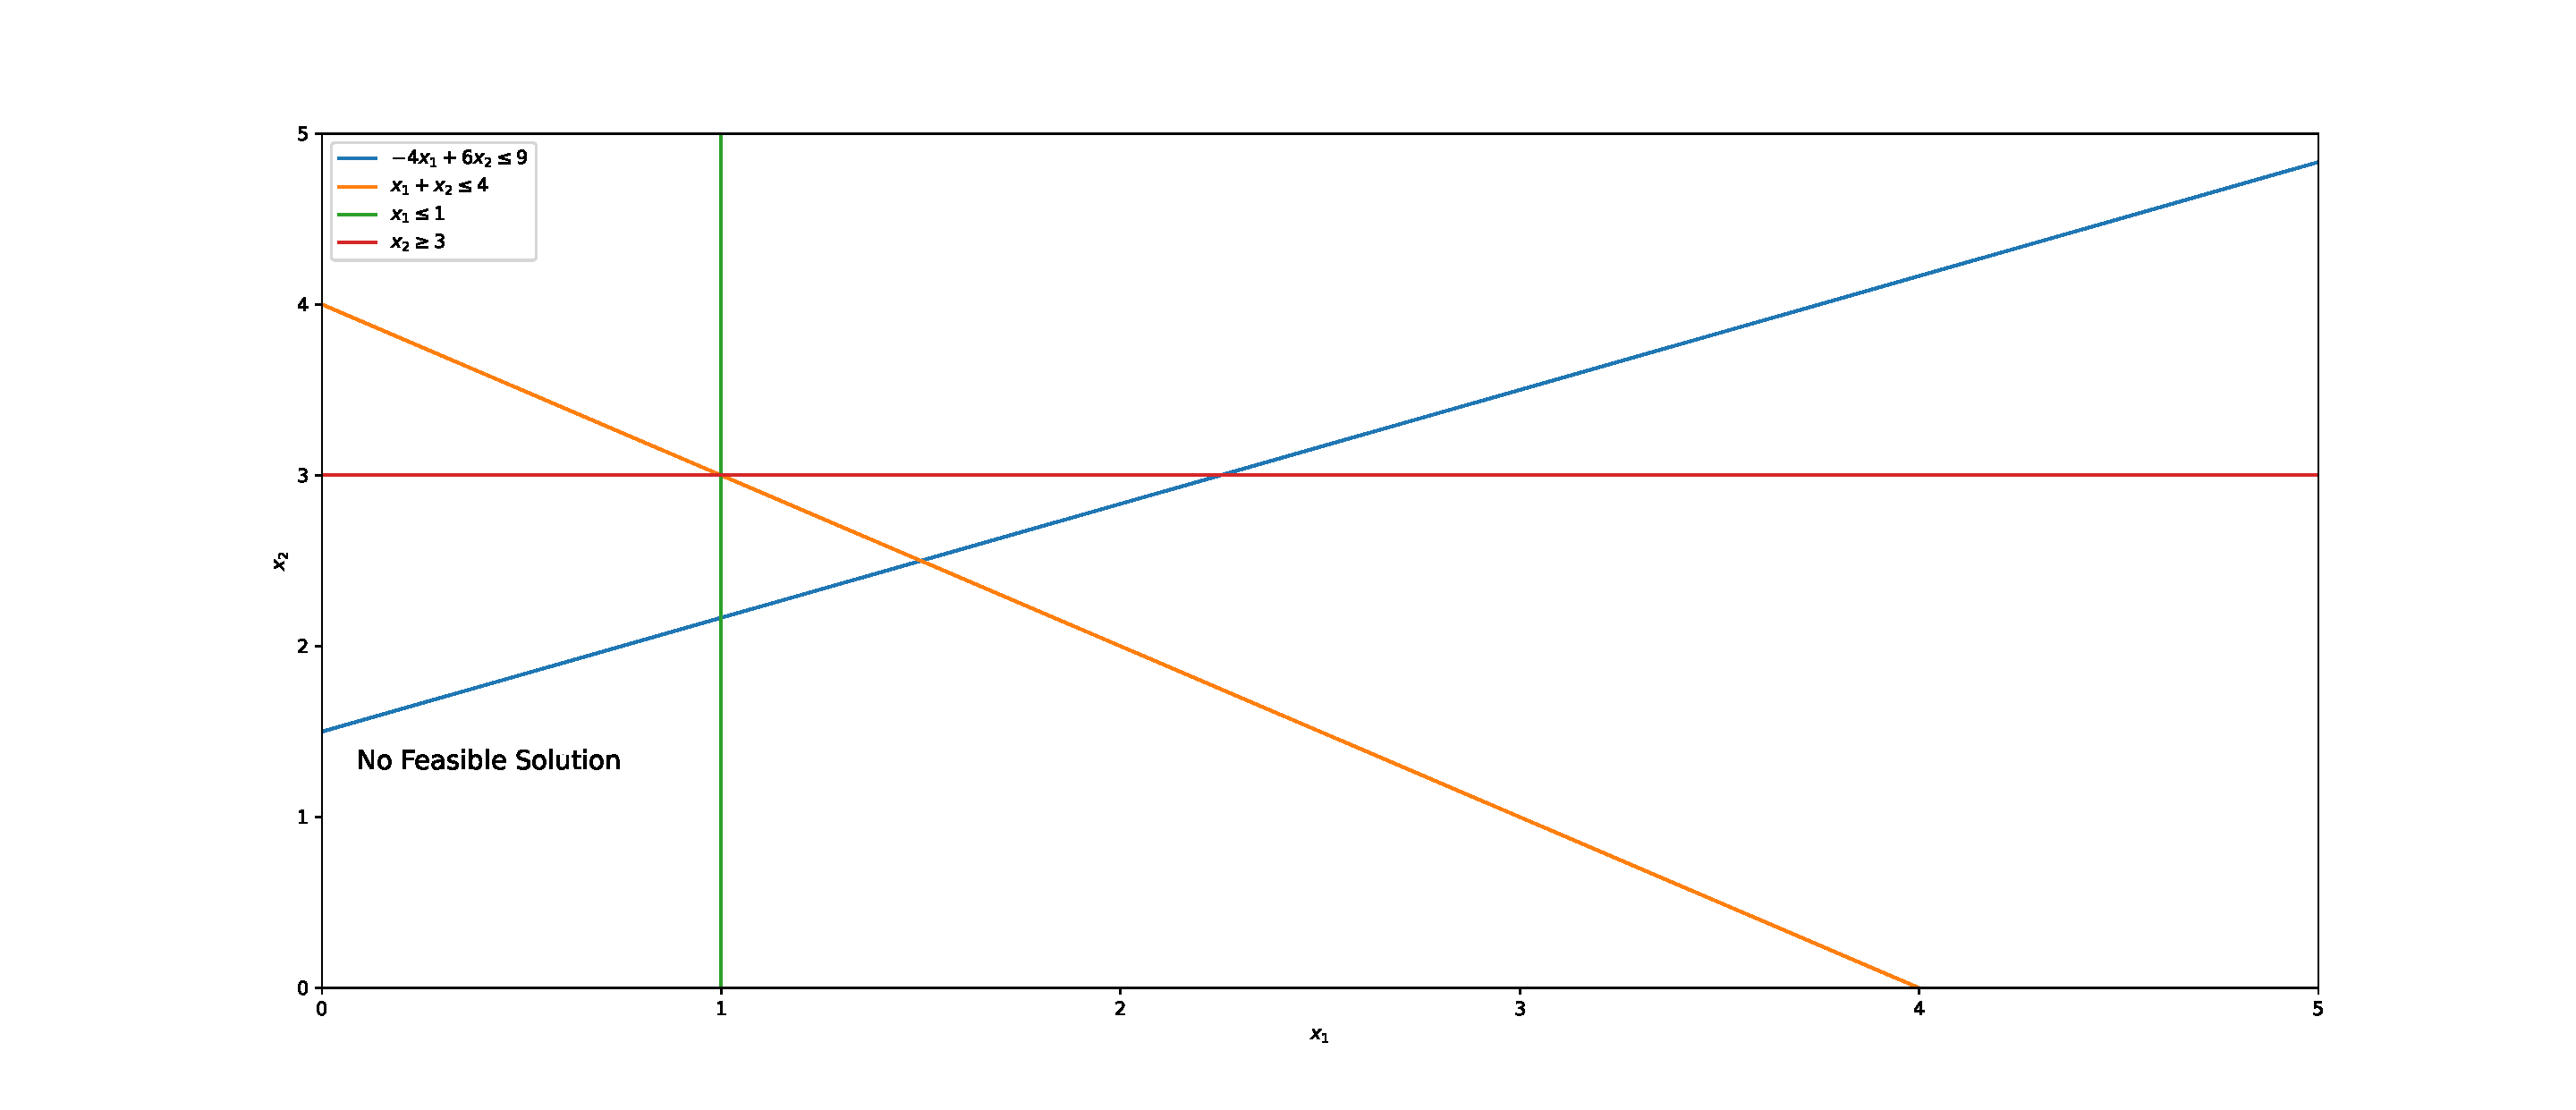
\includegraphics[width = \textwidth]{Exercice/PY/EX2/ex2.6.pdf}
\end{center}
\begin{center}
    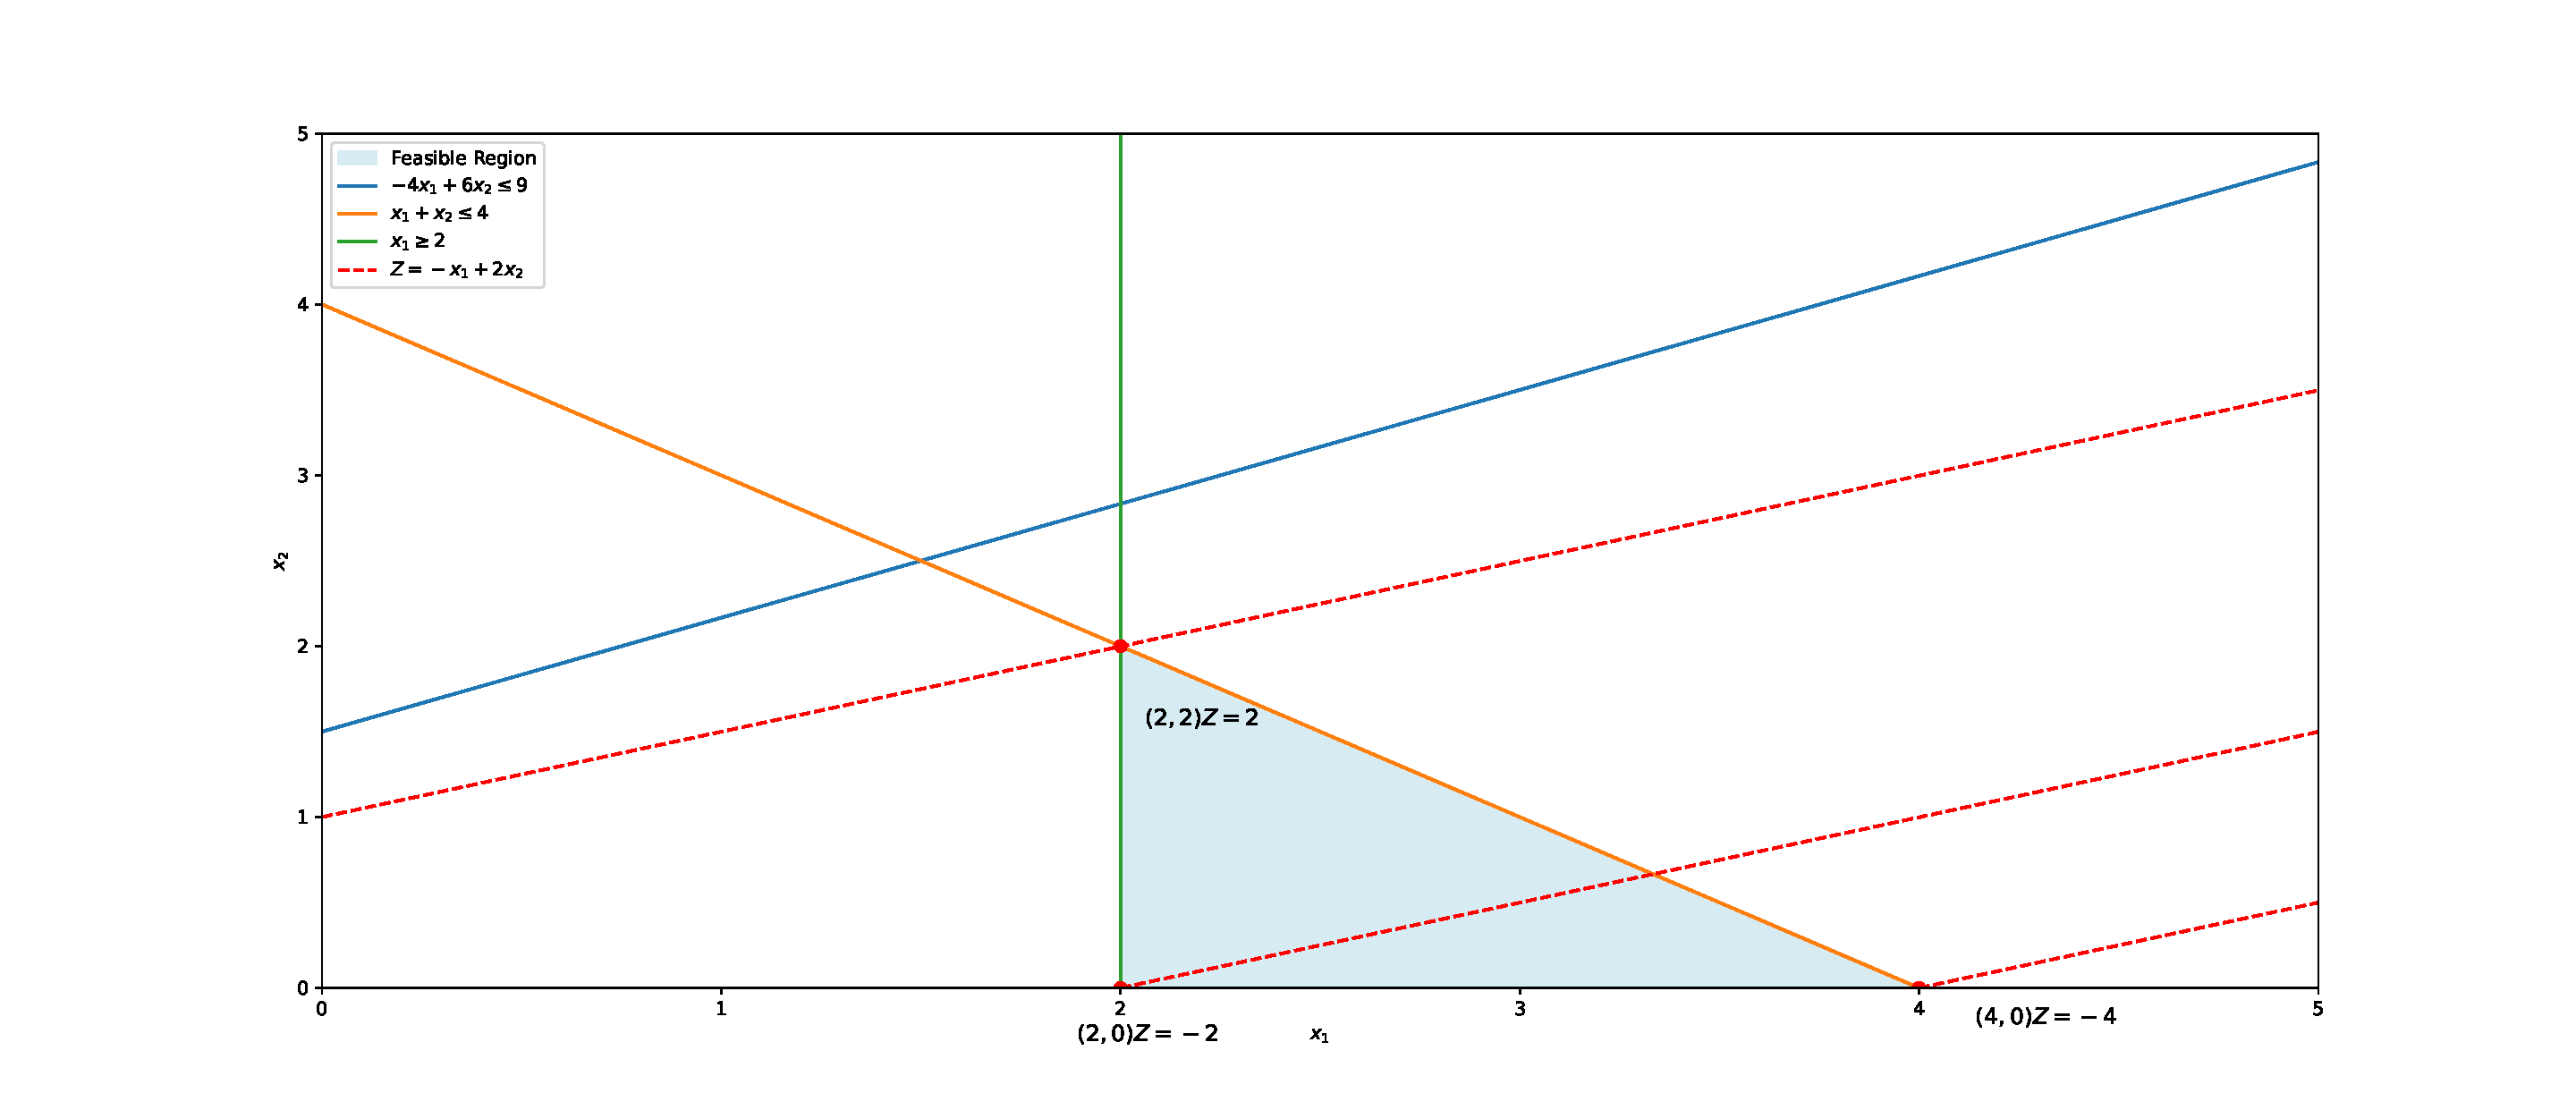
\includegraphics[width = \textwidth]{Exercice/PY/EX2/ex2.7.pdf}
\end{center}


\end{document}
